
\section{Impact of pile-up}

\label{sec:pileup}

The discussion so far has not accounted for the effects of
pile-up (PU), which are known to be very important at the HL-LHC.
%
In this section, we show how our qualitative results, in particular
the enhanced discrimination provided by the MVA, are robust
in the presence of realistic PU conditions.


First of all we describe the simulation of realistic
PU conditions at the HL-LHC, and discuss the settings of
the PU subtraction strategy that we adopt.
%
Then we present the validation of the PU subtraction,
and compare a number of distributions, including substructure variables,
with and without PU.
%
Finally we revisit the MVA analysis of Sect.~\ref{sec:mva}, and
show that our qualitative conclusions are robust
in the presence of realistic PU conditions.
%
As we will show now, a signal significance for
Higgs production in the $4b$ final state
of up to $S/\sqrt{B}\simeq 4$
can be achieved at the HL-LHC even accounting for PU.


\subsection{PU subtraction with {\tt SoftKiller}}

To study the impact of PU in our analysis,
a large number
of Minimum Bias (MB) events,
including Multiple Parton Interactions (MPI),
have been added to the signal
and background samples described in Sect.~\ref{mcgeneration}.
%
We have explored two scenarios for the amount of PU expected
at the HL-LHC, one with a mean number of
PU vertices of $\la n_{\rm PU}\ra=80$, and another
with $\la n_{\rm PU}\ra=150$.
%
MB events have been generated with {\tt Pythia8} using
the Monash 2013 tune.
%
We have generated a total of 100M minimum-bias events, which are
then randomly superimposed to the hard-scattering events.

In order to subtract the PU, a large number of techniques
have been proposed recently~\cite{Cacciari:2009dp,TheATLAScollaboration:2013pia,Butterworth:2008iy,Cacciari:2007fd,Krohn:2009th,Krohn:2013lba,Ellis:2009me,Bertolini:2014bba,Cacciari:2014gra,Cacciari:2014jta,Berta:2014eza,Larkoski:2014wba}.
%
In this work, PU  will be subtracted by means
of the the {\tt SoftKiller} (SK)
method~\cite{Cacciari:2014gra}, as implemented in {\tt FastJet}.
%
Let us note however that
a systematic optimization of the PU subtraction strategy is beyond
the scope of this work, and in particular that further
improvements over the results presented below is feasible
with further tuning of the PU subtraction.


The idea underlying {\tt SoftKiller} is based on eliminating particles
below a given cut-off in their transverse momentum, $p_T^{\rm (cut)}$, whose
value is dynamically determined in a way that makes the event-wide
transverse-momentum flow density $\rho$ vanish.
%
This $p_T$ flow density is defined as
\be
\rho\equiv{\rm median}_i \Bigg\{ \frac{p_{Ti}}{A_i}\Bigg\} \, ,
\ee
where the median is computed over all the patches $i$ with area
$A_i$ and transverse momentum $p_{Ti}$ in which the $\lp \eta,\phi\rp$ plane
is partitioned.
%
From its definition, we observe that the value of $p_T^{(\rm cut)}$
will be dynamically raised until half of the patches have $\rho=0$.

The size and number of these patches is a free parameter of the algorithm -
here we will use square patched with length $a=0.4$.
%
We restrict ourselves to the central rapidity interval,
$\eta \in \lc -2.5, 2.5\rc$, for the estimation of the
$p_T$ flow density $\rho$, which is the region relevant
for the present analysis.
%
In this work, the {\tt SoftKiller} method is applied
to particles at the end of the parton shower, before
the jet clustering stage.

\subsection{Validation of the PU subtraction}

Now we turn to validate our PU subtraction strategy.
%
To this end, we compare different kinematical distributions
in the three relevant cases:
cases:
\begin{itemize}
\item without any PU,
\item adding PU, but without any PU subtraction,
  \item adding PU, followed by the {\tt SoftKiller} subtraction.
\end{itemize}
As we will show now, {\tt SoftKiller} exhibits a reasonable
performance in PU subtraction.
%
We will also see that the boosted category is less affected
by PU than the resolved category, as expected from the higher
$p_T$ threshold in the corresponding selection cuts.

Let us begin by comparing
a number of signal distributions with
and without PU, with $\la n_{\rm PU}\ra=80$ in the former
case.
%
In Fig.~\ref{fig:m_H_PU} we show the invariant mass distribution
of the leading and subleading Higgs candidates. in the boosted
and resolved categories.
%
These distributions are plotted after the $b$-tagging, that is,
before they are used as input to the MVA.
%
As we can see, in the boosted category, the residual effects of PU
after the {\tt SoftKiller} subtraction are very mild in these
distributions, with the position of the Higgs mass peaks essentially
unchanged.
%
The effects are more important for the resolved category, where PU
shifts the Higgs peak by an amount $\Delta m_h \simeq 5$ GeV.

%%%%%%%%%%%%%%%%%%%%%%%%
\begin{figure}[t]
  \begin{center}
      \vspace{-1cm}
      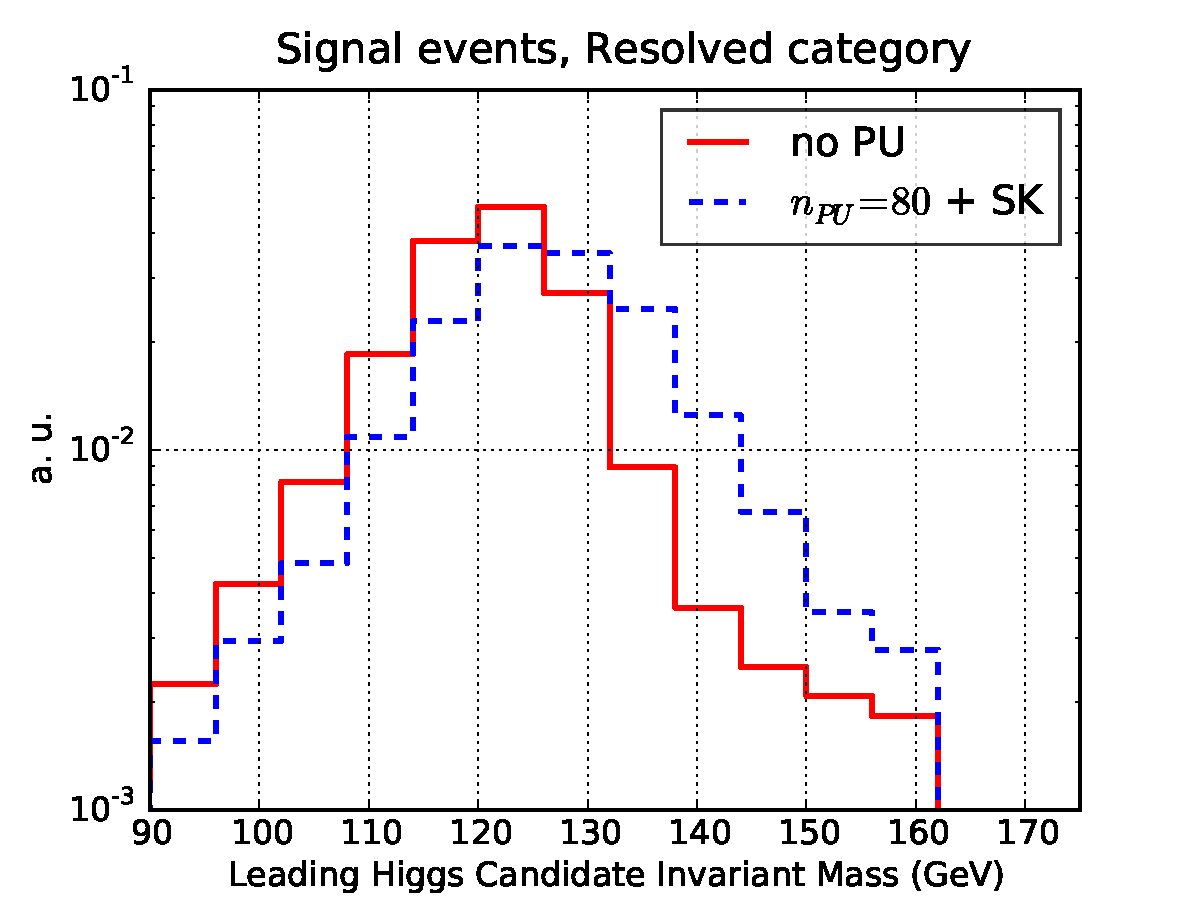
\includegraphics[width=0.49\textwidth]{plots/m_H0_res_comp.pdf}
      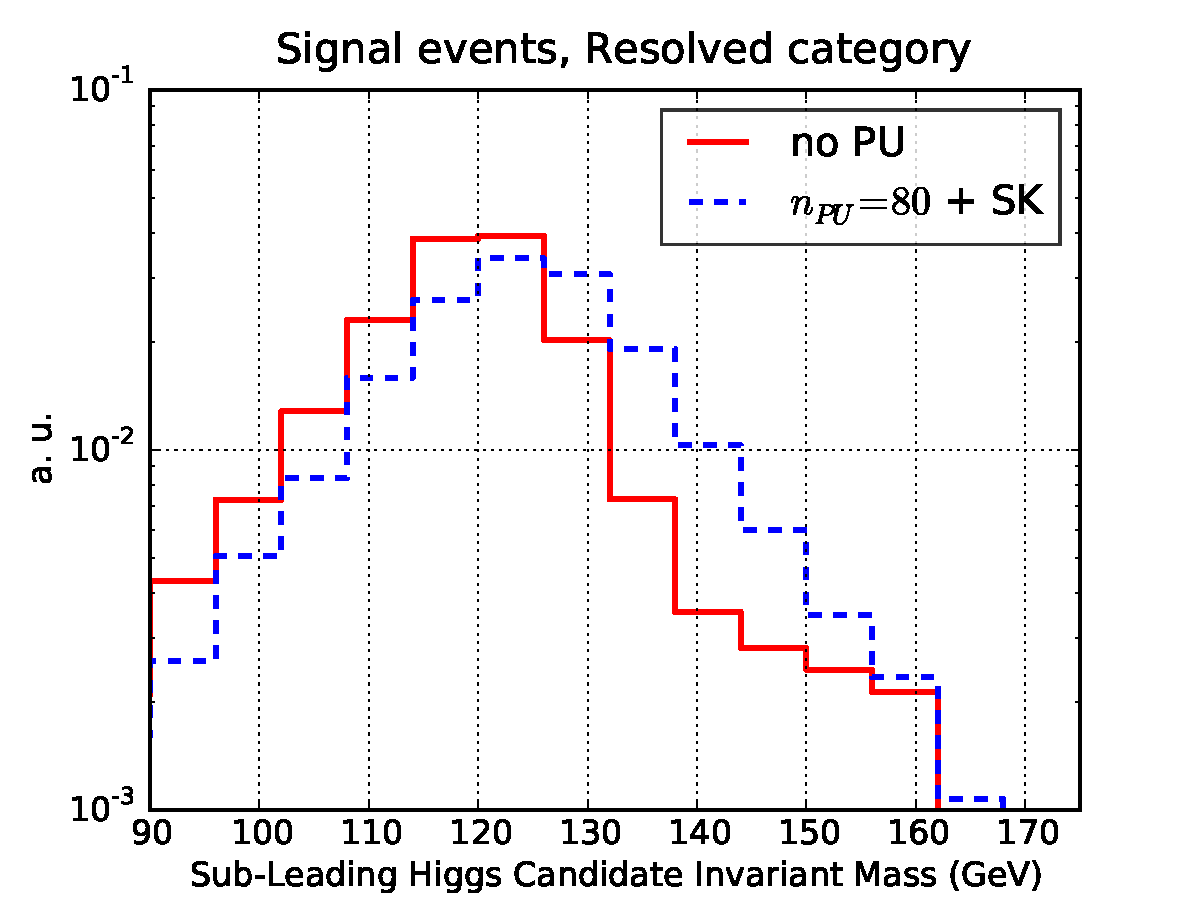
\includegraphics[width=0.49\textwidth]{plots/m_H1_res_comp.pdf}
      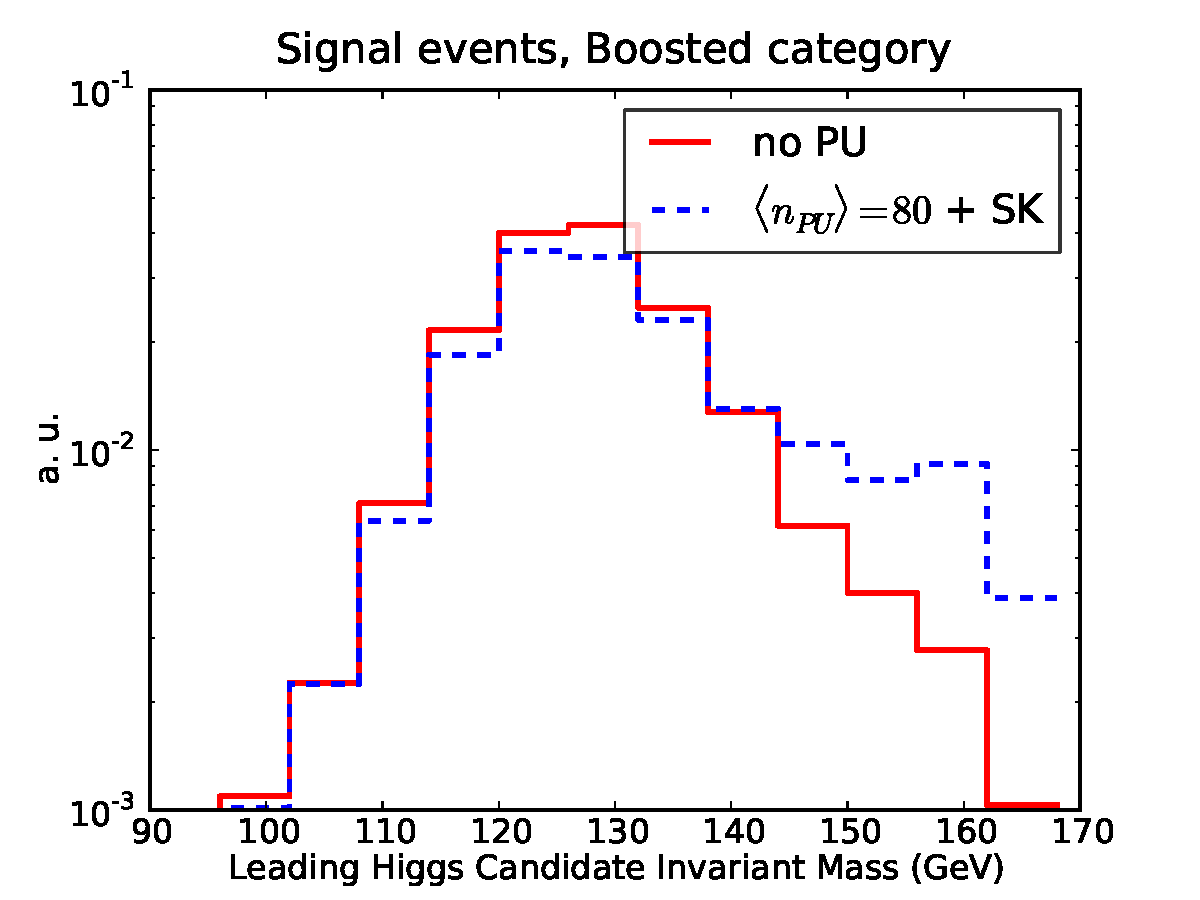
\includegraphics[width=0.49\textwidth]{plots/m_H0_bst_comp.pdf}
      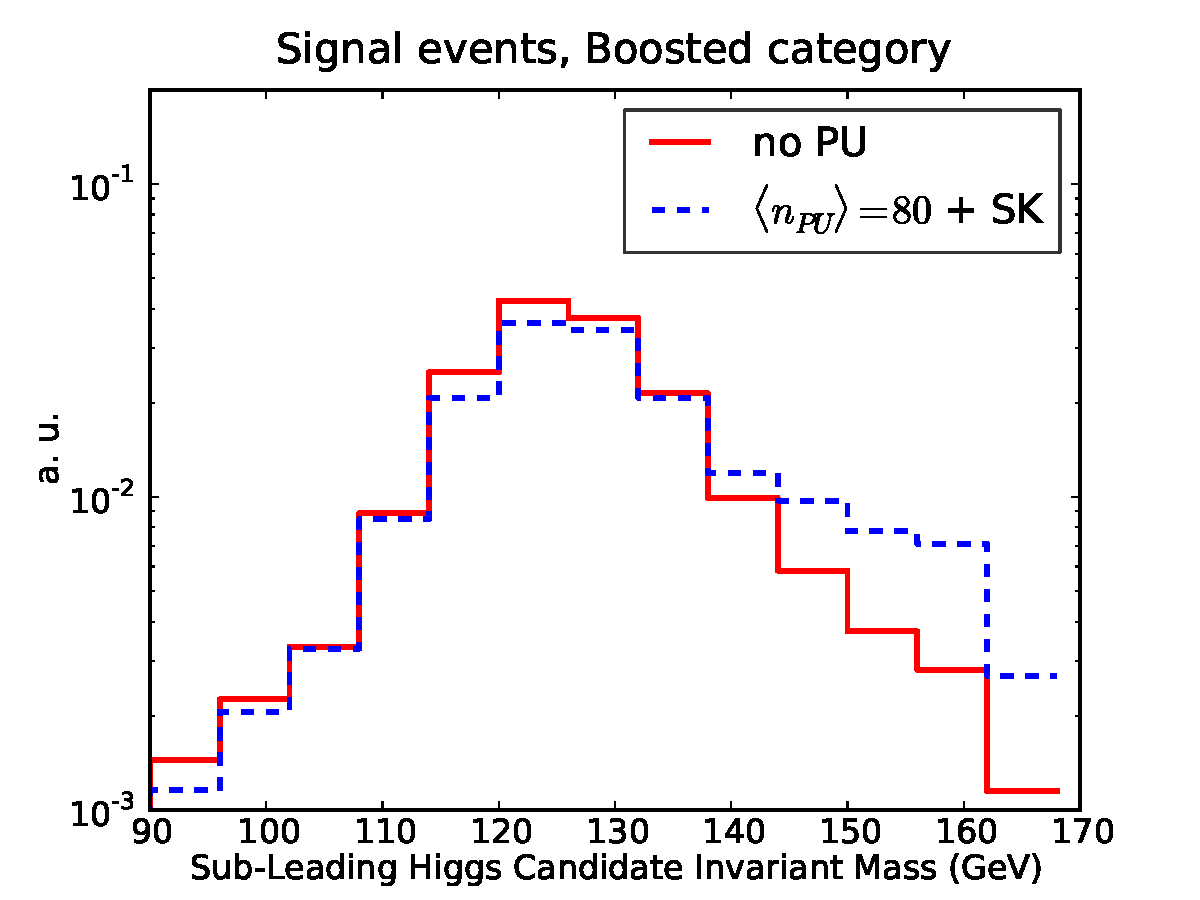
\includegraphics[width=0.49\textwidth]{plots/m_H1_bst_comp.pdf}
  \caption{\small
    Comparison of the invariant mass distributions of the leading (left plots)
    and subleading (right plots) Higgs candidates in the resolved
    (upper plots) and boosted (lower plots) categories,
    without PU and with $\la n_{PU}\ra=80$ subtracted with {\tt SoftKiller}.
}
\label{fig:m_H_PU}
\end{center}
\end{figure}
%%%%%%%%%%%%%%%%%%%%%%%

Next we compare the transverse momentum of the leading Higgs
candidate, $p_t^{h_1}$ and the invariant mass of the di-Higgs system
$m_{hh}$, in Fig.~\ref{fig:mHH_PU}, both for the boosted and
for the resolved categories.
%
In the case of the $p_T$, the differences between the resolved
and boosted selection cuts can be clearly observed.
%
The effect of PU is negligible in the boosted case, and small
in the resolved case, except for large $p_T$ values.
%
For the case of the $m_{hh}$ distribution, similar conclusions
apply.
%
Note that this latter observable is particularly sensitive
of BSM dynamics.


%%%%%%%%%%%%%%%%%%%%%%%%
\begin{figure}[t]
  \begin{center}
    \vspace{-1cm}
  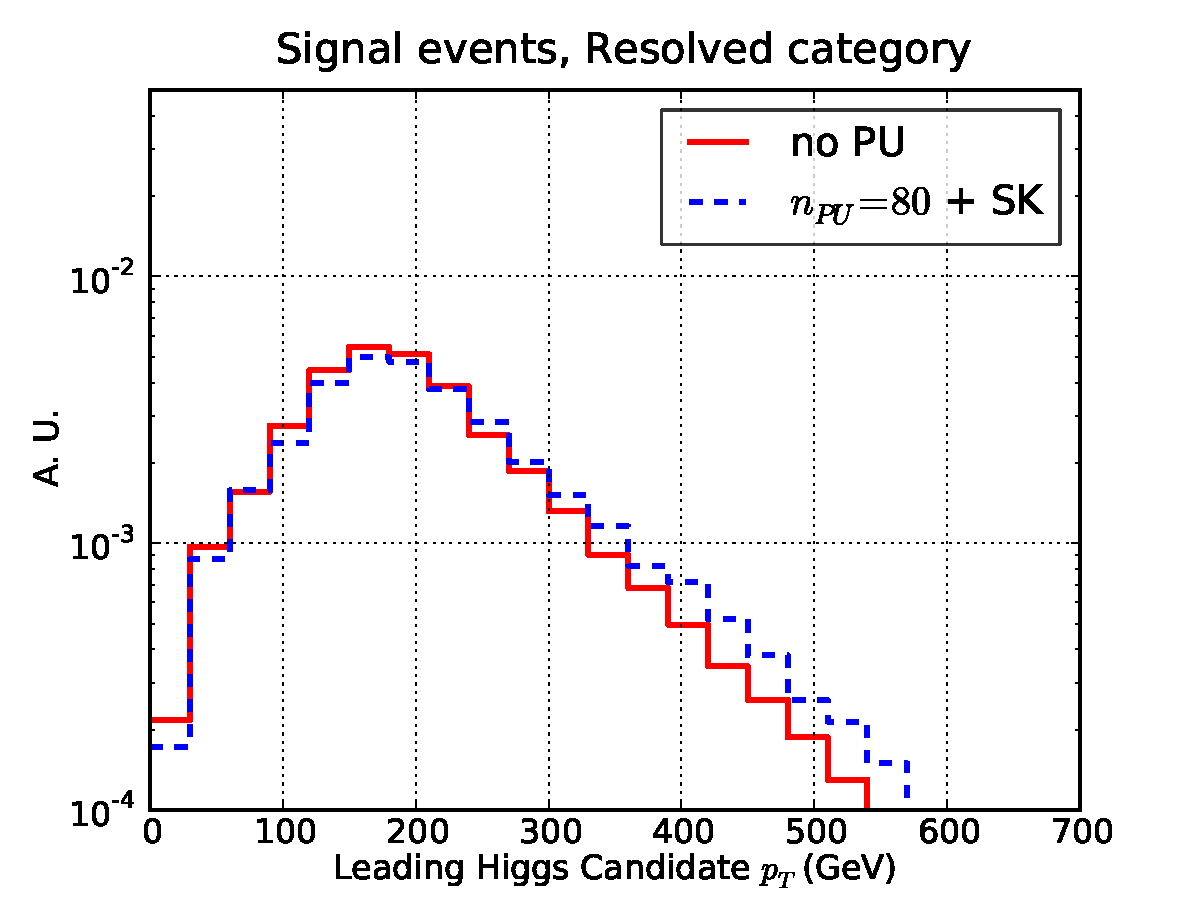
\includegraphics[width=0.49\textwidth]{plots/pt_H0_C2_res_comp.pdf}
  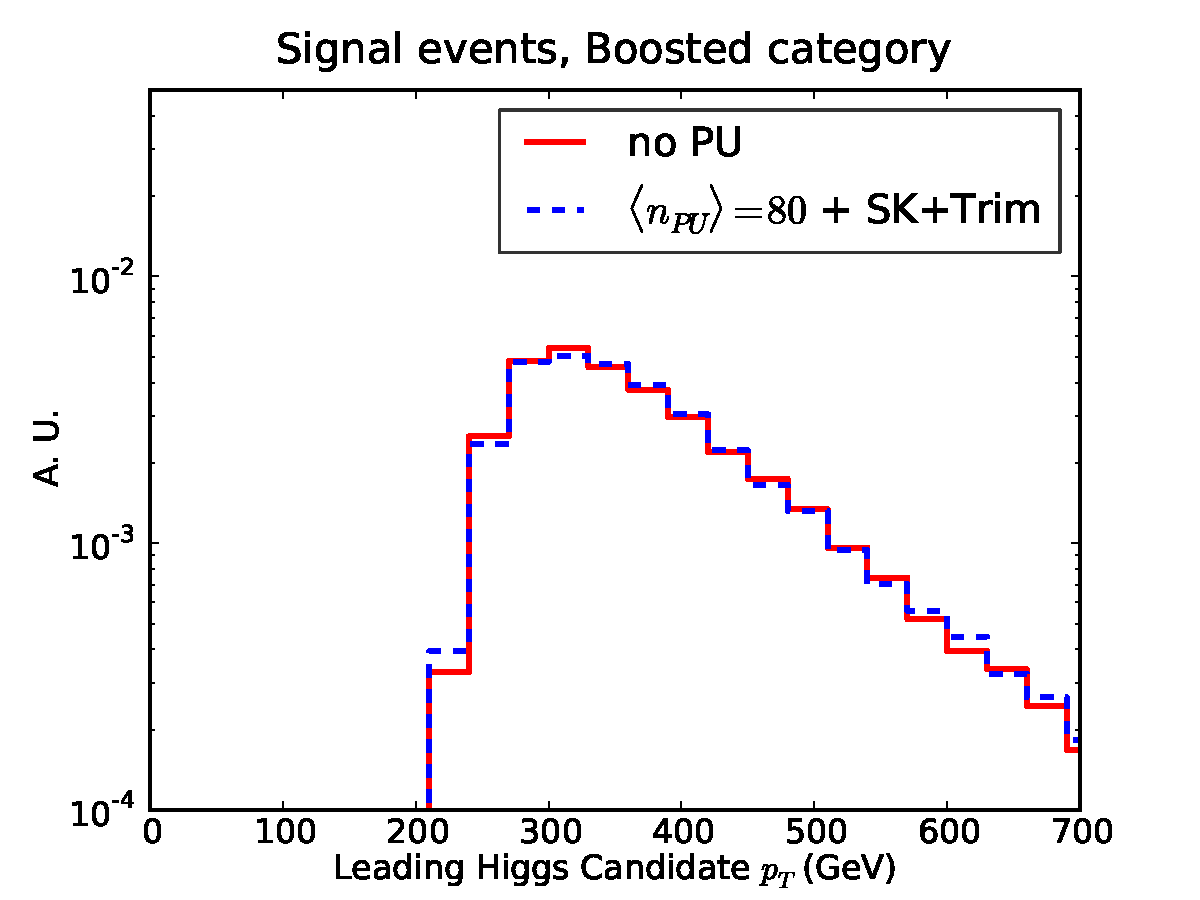
\includegraphics[width=0.49\textwidth]{plots/pt_H0_C2_bst_comp.pdf}
  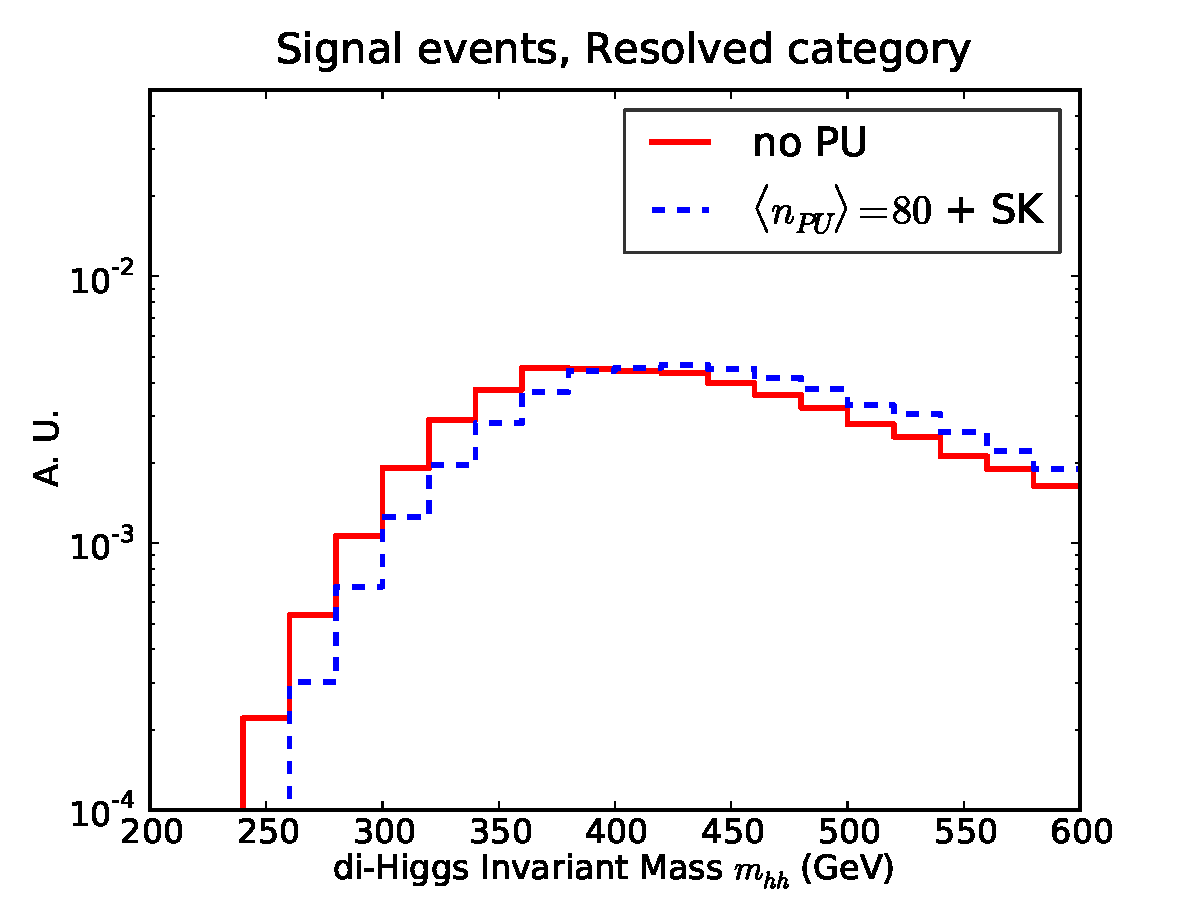
\includegraphics[width=0.49\textwidth]{plots/m_HH_C2_res_comp.pdf}
  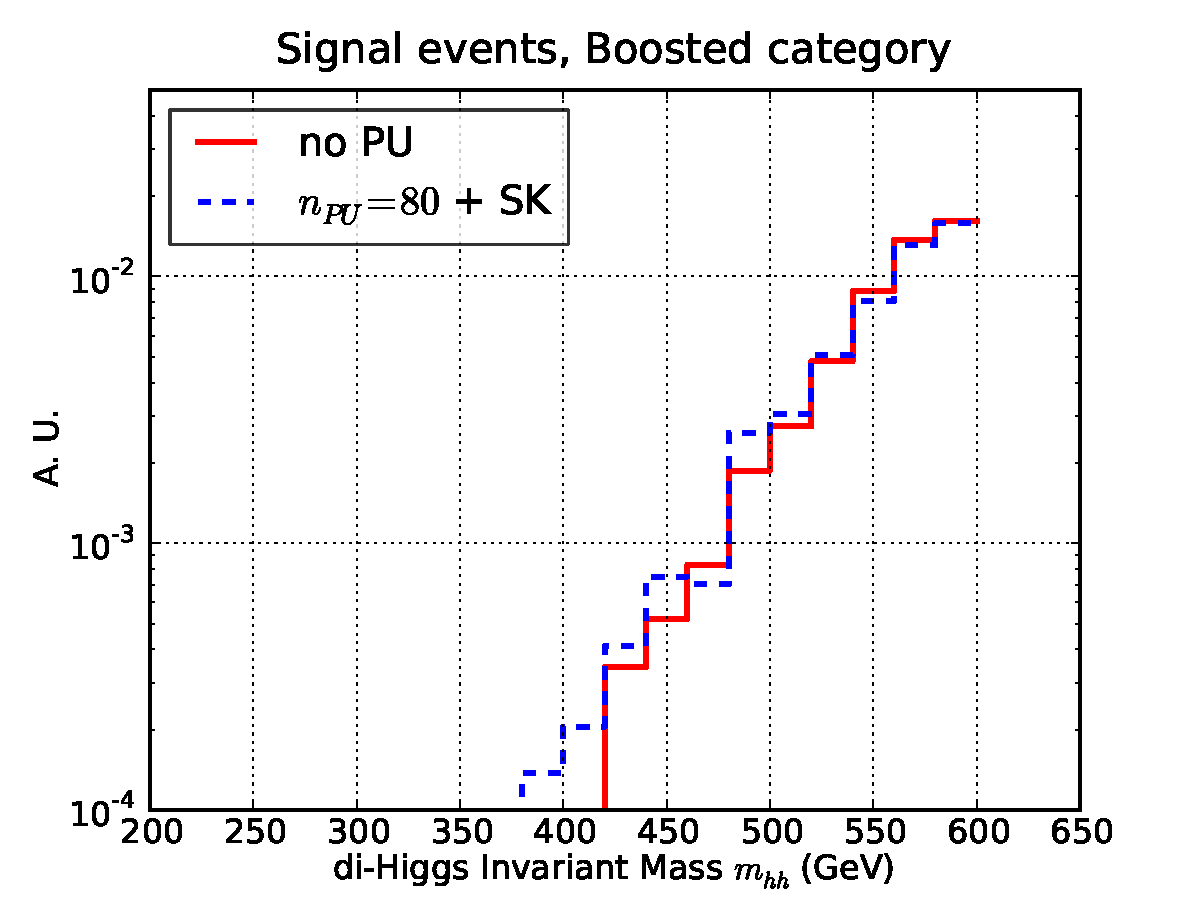
\includegraphics[width=0.49\textwidth]{plots/m_HH_C2_bst_comp.pdf}
  \caption{\small
    Comparison of the transverse momentum $p_T^h$ of the leading
    Higgs candidate (upper plots) and of the invariant mass $m_{hh}$
    of the di-Higgs system (lower plots) in the resolved
    (left plots) and boosted (right plots) categories,
    without PU and with $\la n_{PU}\ra=80$ subtracted with {\tt SoftKiller}.
}
\label{fig:mHH_PU}
\end{center}
\end{figure}
%%%%%%%%%%%%%%%%%%%%%%%

Then we assess the impact of PU in some of the substructure variables
used as input to the MVA in the boosted category.
%
In particular we consider the subjetiness variable,
$\tau_{21}$, and the ratio
of energy correlation functions $D_2^{(\beta)}$,
corresponding to the the leading Higgs candidate.
%
This comparison is illustrated in Fig.~\ref{fig:Substructure_PU}.
%
As can be seen, these substructure variables, which
as demonstrated before carry a very substantial
discrimination power, are relatively unaffected by PU.
%
Therefore, we don't expect a substantial loss of discrimination
power due to PU effects in our analysis.


%%%%%%%%%%%%%%%%%%%%%%%%
\begin{figure}[t]
  \begin{center}
    \vspace{-1cm}
  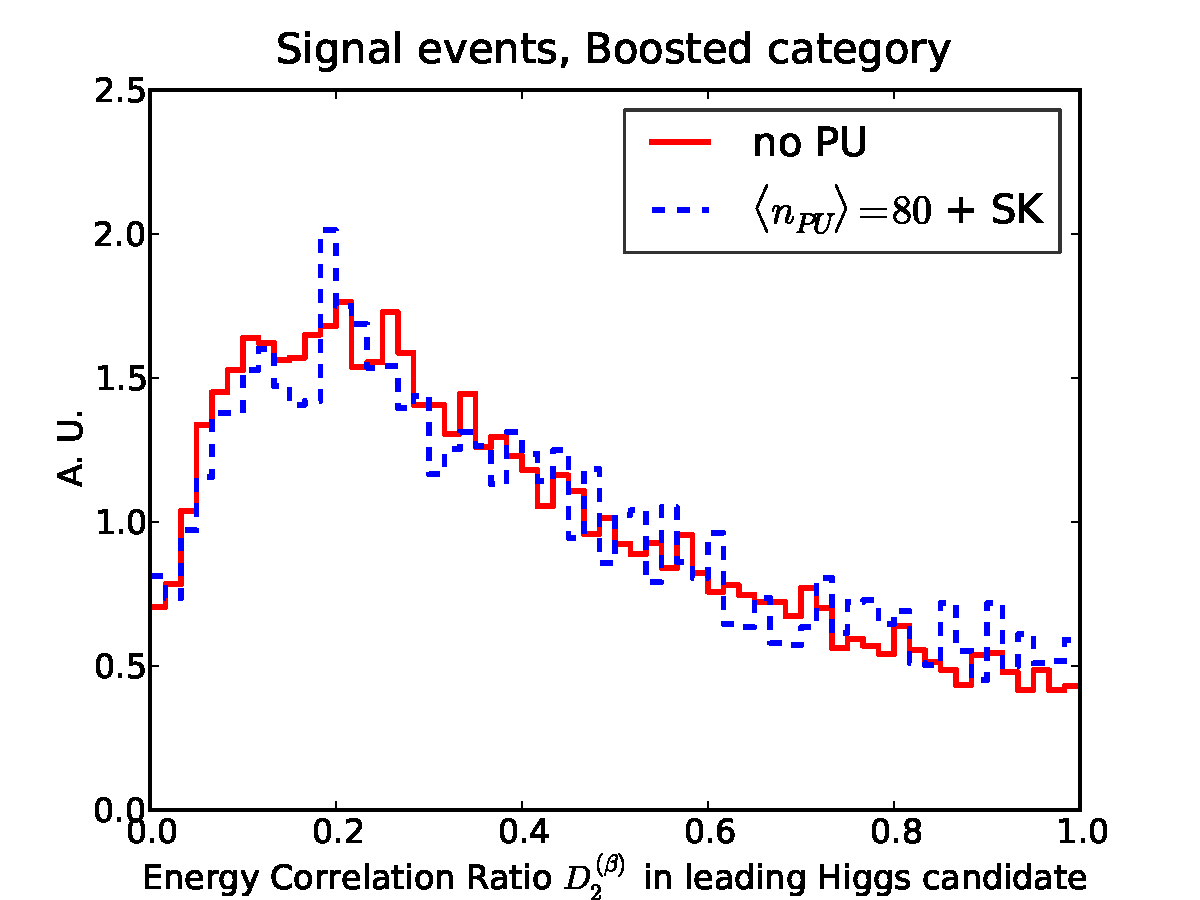
\includegraphics[width=0.49\textwidth]{plots/D2_h0_bst_comp.pdf}
  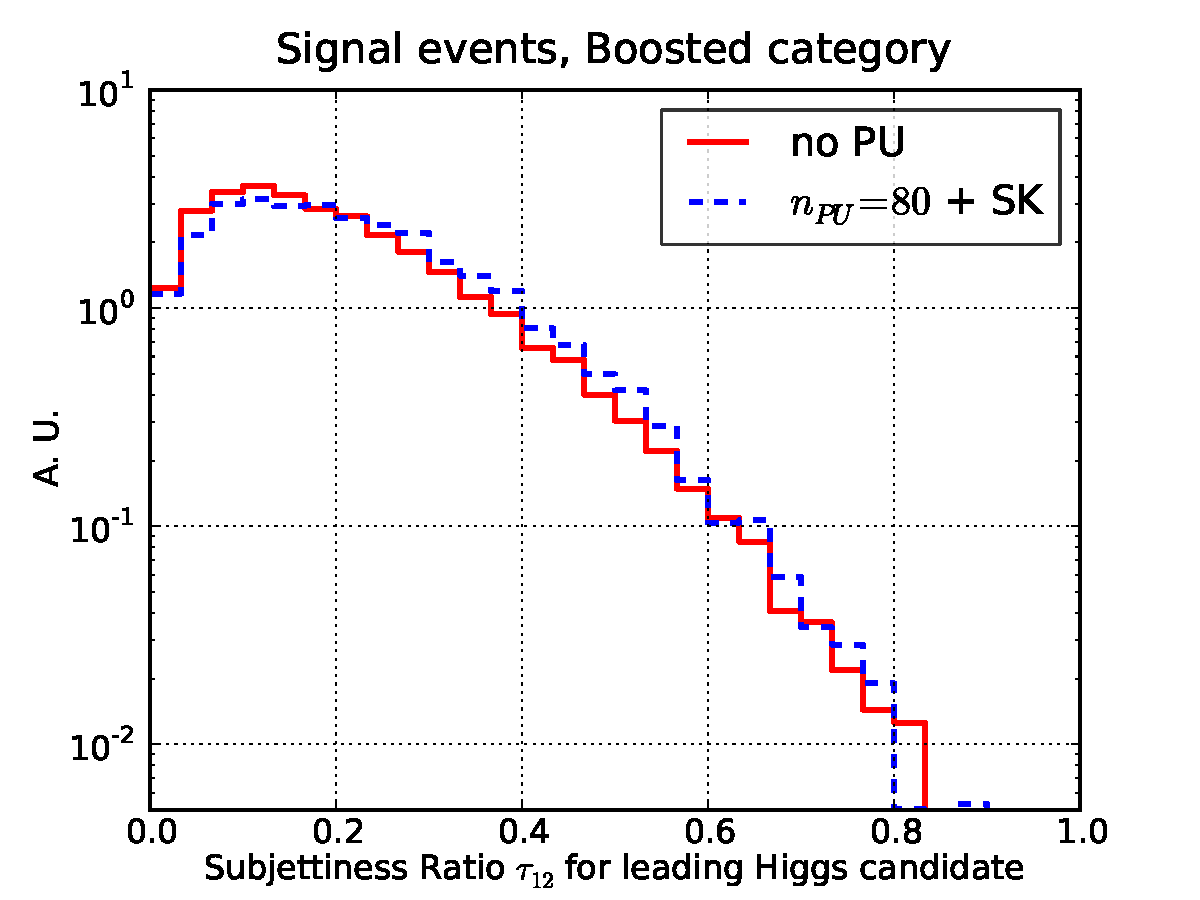
\includegraphics[width=0.49\textwidth]{plots/tau21_h0_bst_comp.pdf}
   \caption{\small
     Comparison of the substructure variables $D_2^{(\beta)}$ (left)
     and $\tau_{21}$ (right)
     for the leading Higgs candidate in the boosted category,
   without PU and with $\la n_{PU}\ra=80$ subtracted with {\tt SoftKiller}.
}
\label{fig:Substructure_PU}
\end{center}
\end{figure}
%%%%%%%%%%%%%%%%%%%%%%%


Up to know we have restricted ourselves to the study of the impact of PU
on signal distributions.
%
We now assess how the signal over background discrimination can be affected
in the presence of realistic PU conditions.
%
First of all let us consider the boosted category.
%
In Fig.~\ref{fig:signal-vs-back-boosted} we compare
various kinematical distributions for signal and background events,
     with and without PU: the invariant mass and the $p_T$ of the leading
     Higgs candidate, and the $\tau_{21}$ and $D^{(\beta)}_2$ substructure variables.
     %
     All these distributions correspond to the boosted category.
     %
     While for signal distributions the effects of PU after SK subtraction are small,
     differences are more marked for the background distributions, where
     the shapes of the distributions with and without background can be substantially
     different.
     %
     We note however that the fact that signal and background distribution exhibit
     rather different behaviors is maintained in the presence of PU.
     

%%%%%%%%%%%%%%%%%%%%%%%%
\begin{figure}[t]
  \begin{center}
    \vspace{-1cm}
  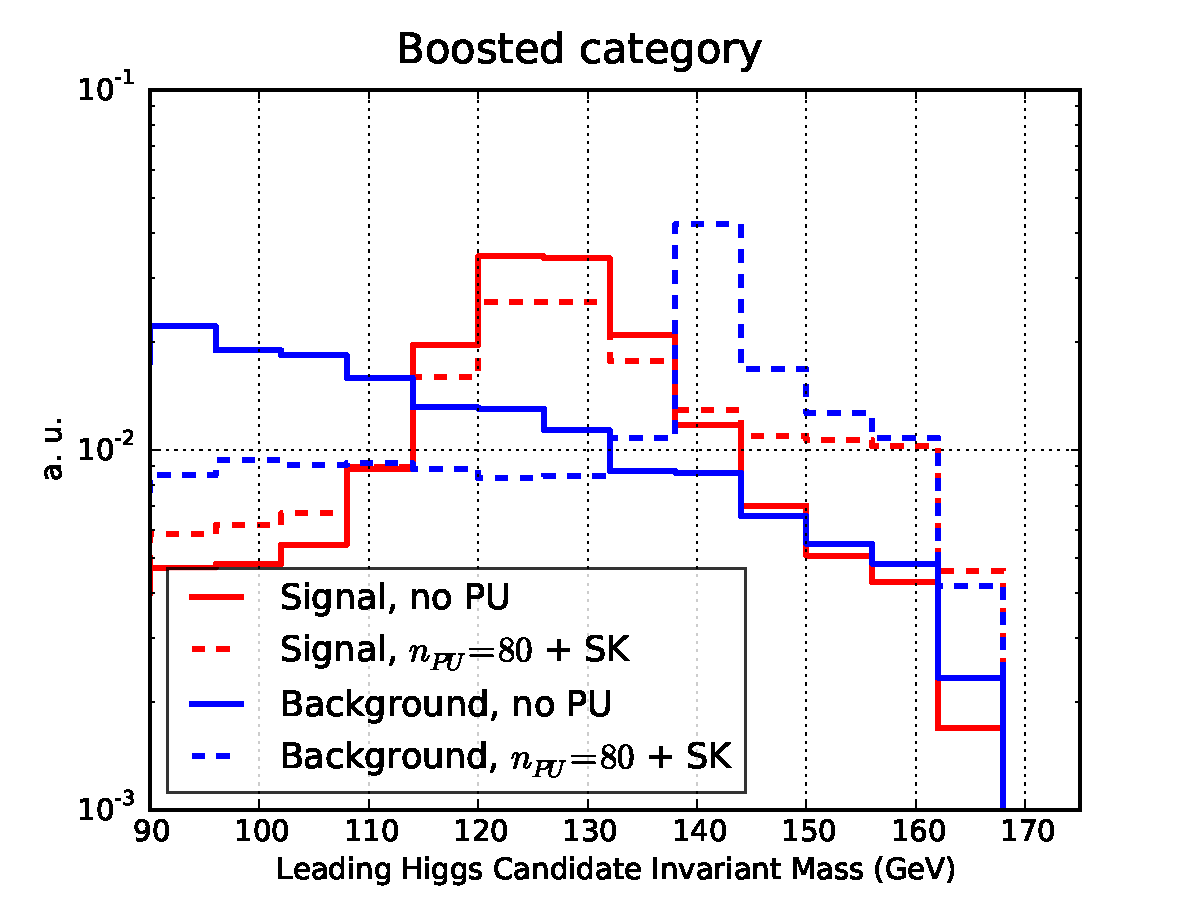
\includegraphics[width=0.49\textwidth]{plots/m_h0_bst_comp_back.pdf}
  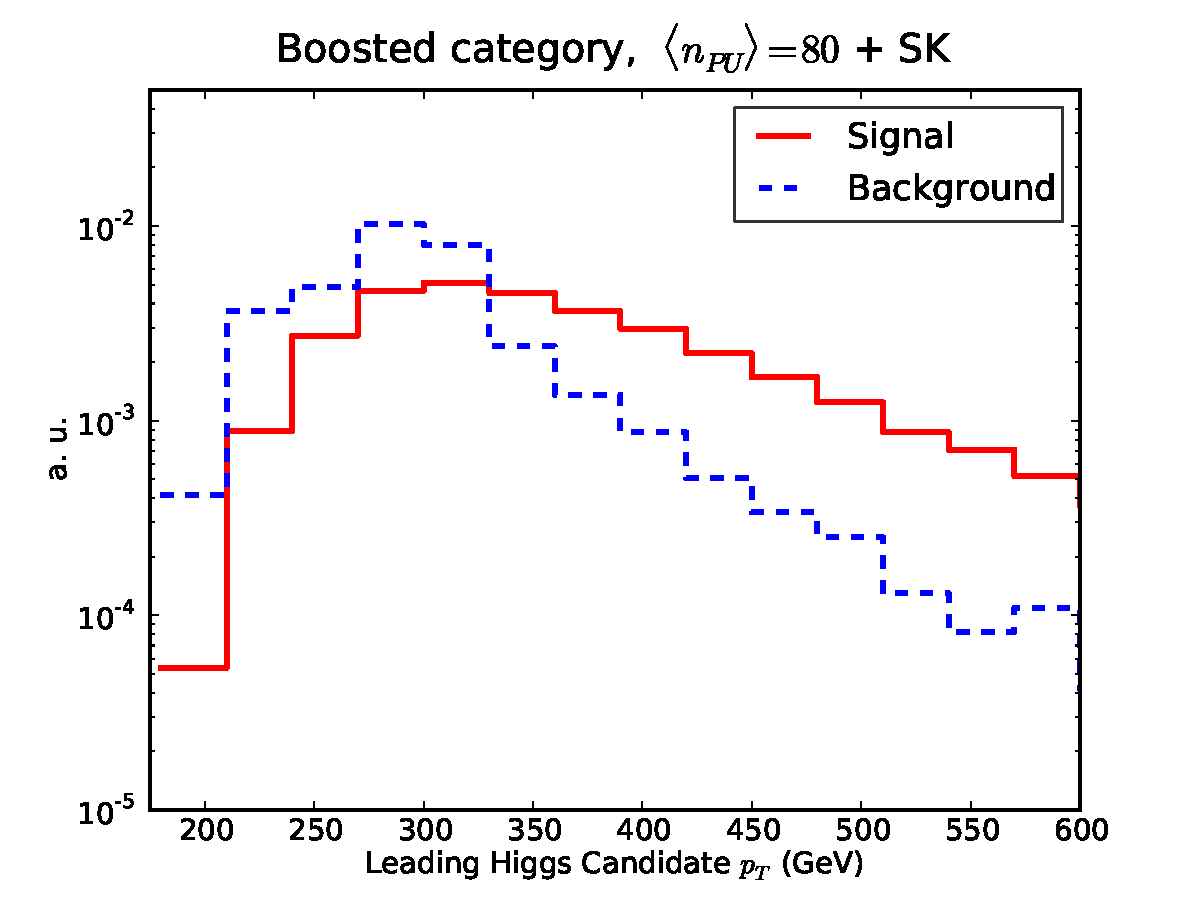
\includegraphics[width=0.49\textwidth]{plots/pt_h0_bst_comp_back.pdf}
   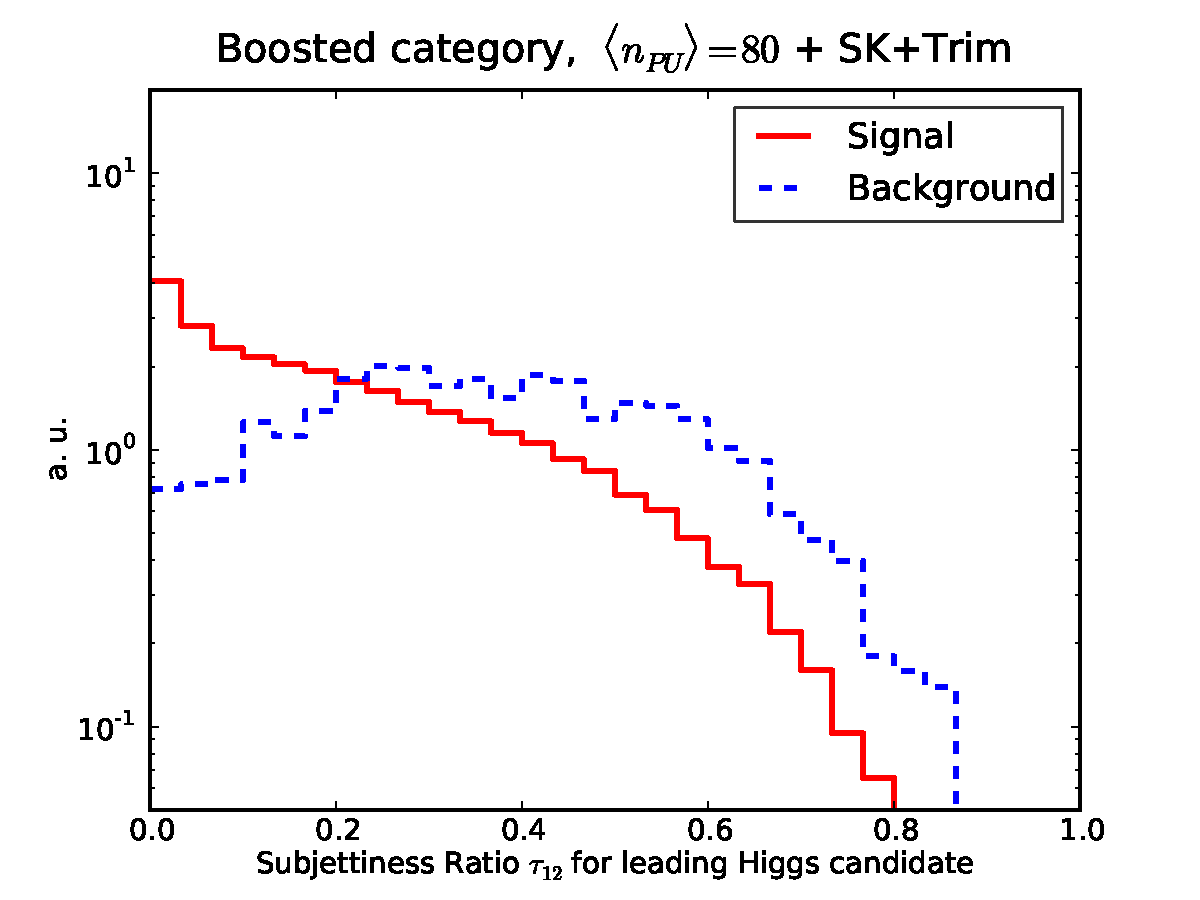
\includegraphics[width=0.49\textwidth]{plots/tau21_h1_bst_comp_back.pdf}
  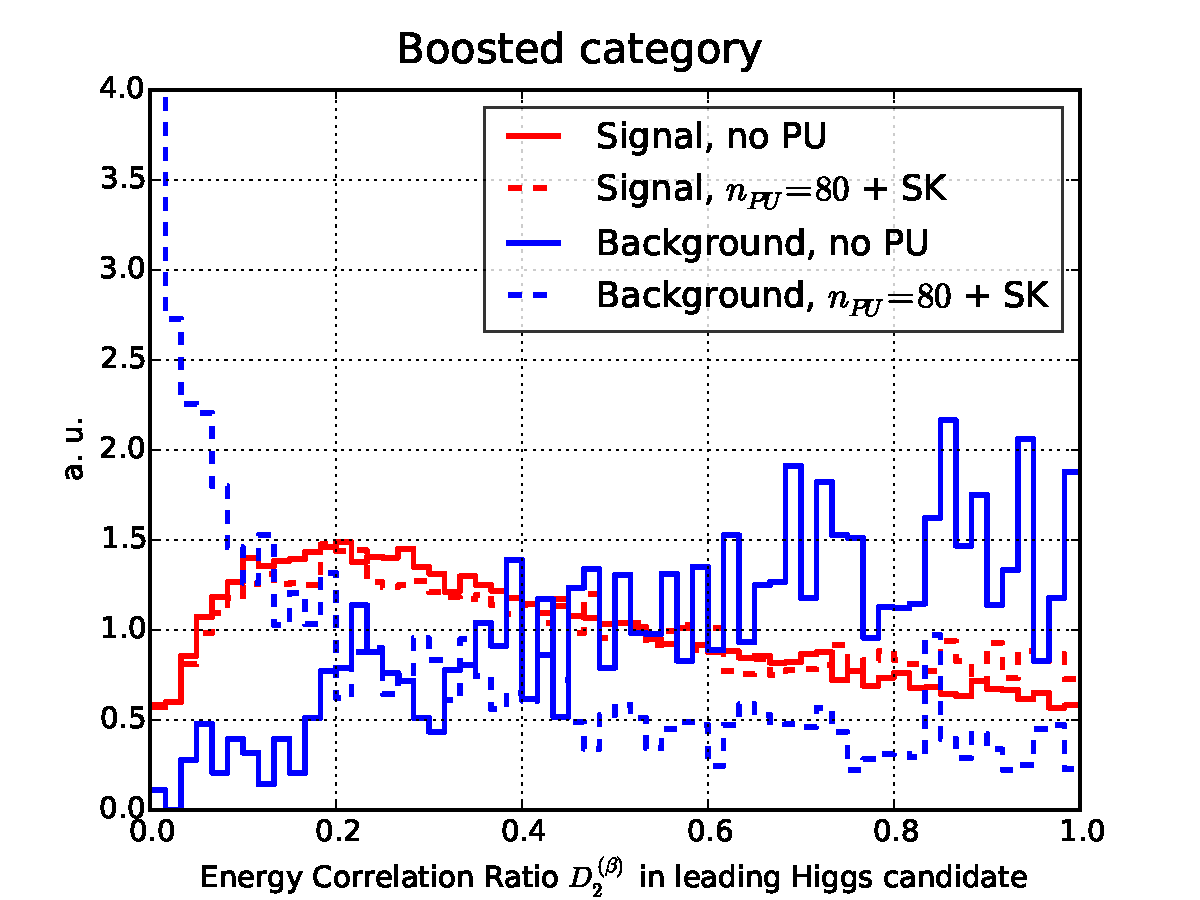
\includegraphics[width=0.49\textwidth]{plots/D2_h0_bst_comp_back.pdf}
   \caption{\small
     Comparison of kinematical distributions for signal and background events,
     with and without PU: the invariant mass and the $p_T$ of the leading
     Higgs candidate, and the $\tau_{21}$ and $D^{(\beta)}_2$ substructure variables.
     %
     All these distributions correspond to the boosted category.
}
\label{fig:signal-vs-back-boosted}
\end{center}
\end{figure}
%%%%%%%%%%%%%%%%%%%%%%%



Now we perform a similar comparison this time for
the resolved category.
%
In Fig.~\ref{fig:signal-vs-back-resolved} we compare
the kinematical distributions for signal and background events,
     with and without PU, for the invariant mass and the $p_T$ of the leading
     Higgs candidate.
     %
     Here the PU-subtracted background distributions appear reasonably close
     to their no PU counterparts.
     %
     Differences between signal and background distributions are maintained after PU
     has been accounted for - we have checked that this is the case
     in general.


%%%%%%%%%%%%%%%%%%%%%%%%
\begin{figure}[t]
  \begin{center}
    \vspace{-1cm}
  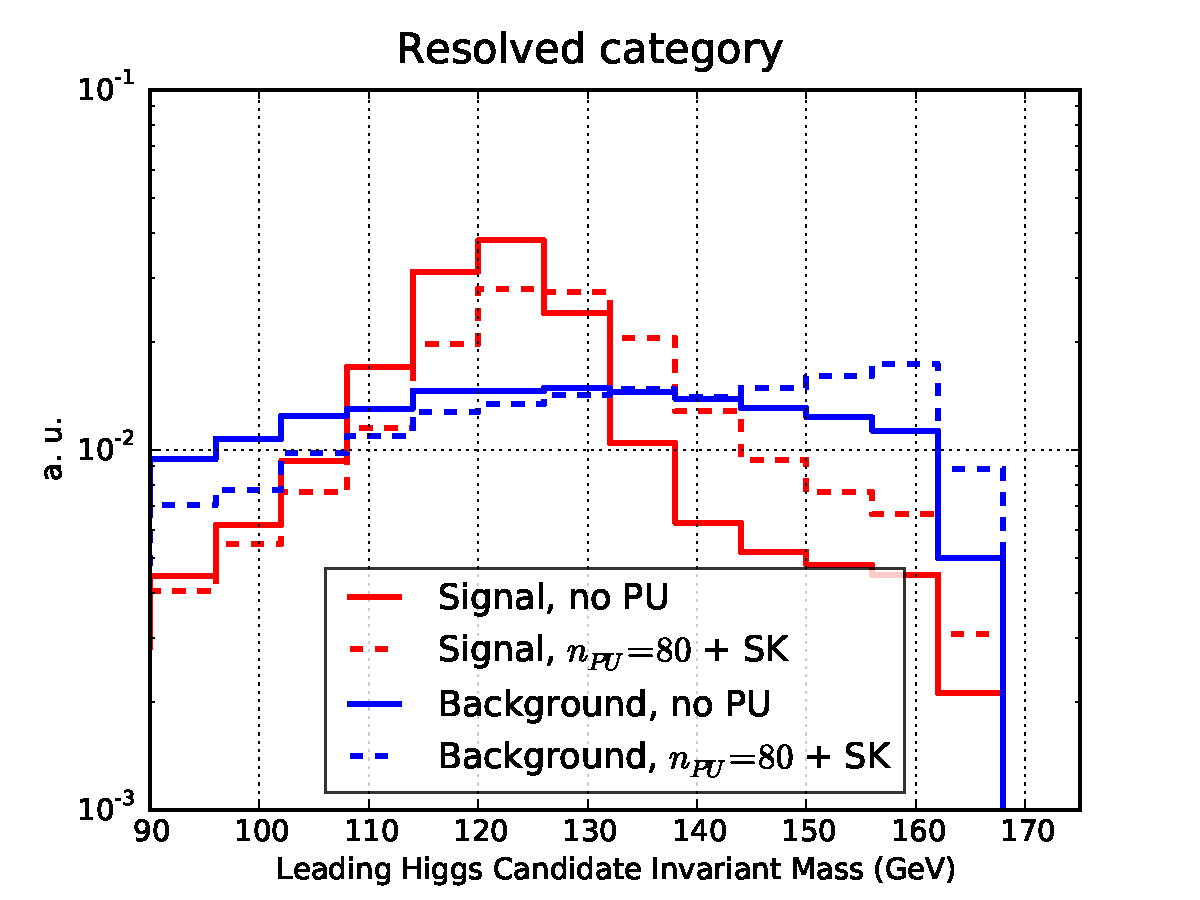
\includegraphics[width=0.49\textwidth]{plots/m_h0_res_comp_back.pdf}
  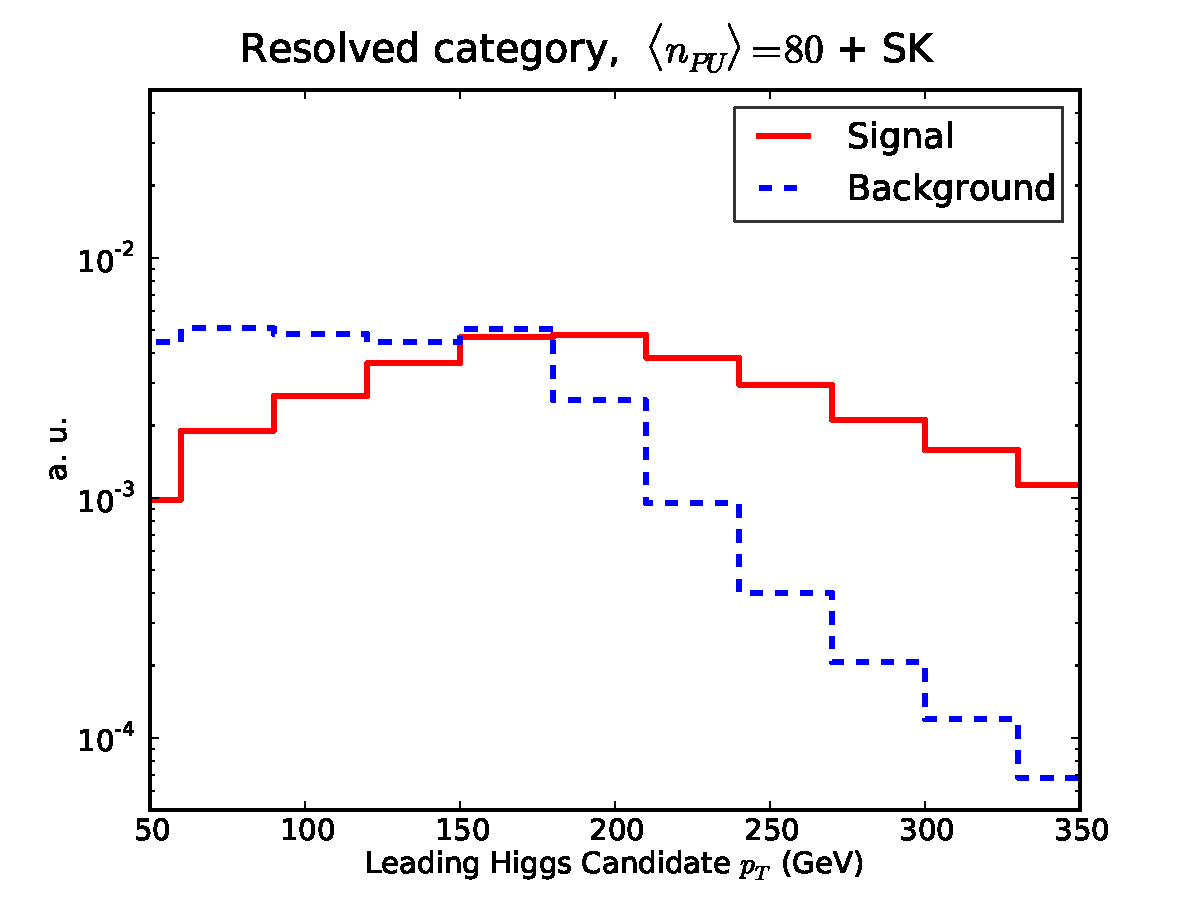
\includegraphics[width=0.49\textwidth]{plots/pt_h0_res_comp_back.pdf}
     \caption{\small
       Same as Fig.~\ref{fig:signal-vs-back-boosted} for the resolved category,
       this time without the jet substructure variables.
}
\label{fig:signal-vs-back-resolved}
\end{center}
\end{figure}
%%%%%%%%%%%%%%%%%%%%%%%

\subsection{Cut-flow}



The corresponding cut-flow tables in the case
of PU subtracted with SK, for $\la n_{\rm PU}\ra=80$,
are shown in Tables~\ref{tab:cutflow_SKPU80_1},
\ref{tab:cutflow_SKPU80_2} and~\ref{tab:cutflow_SKPU80_3},
for the total cross-sections, number of events expected and
signal significance at the HL-LHC, respectively.

%%%%%%%%%%%%%%%%%%%%%%%%%%%%%%%%%%%%%%%%%%%%%%%%%%%%%%%%%%%
\begin{table}[t]
  \centering
  \scriptsize
  \begin{tabular}{|l|cc|cccc|cccc|}
  \hline
\multicolumn{11}{|c|}{Resolved category, $\la n_{\rm PU}\ra=80$+SK}\\
\hline
&  \multicolumn{6}{c|}{Cross-section [pb]} &  &  & &  \\
   &  $hh\to 4b$ &  total bkg  &   $4b$    &  $2b2j$   &   $4j$    &
$t\bar{t}$ &
$S/B_{\rm tot}$ & $S/B_{\rm 4b}$ & $S/\sqrt{B_{\rm tot}}$ & $S\sqrt{B_{\rm 4b}}$ \\
  \hline
  \hline
 C0    & 16  &   $3.1\cdot 10^9$   & $9.0\cdot 10^5$ & $2.1\cdot 10^8$ & $2.9\cdot 10^9$ & $1.8\cdot 10^5$ &   $5.0\cdot 10^{-9}$   & $1.7\cdot 10^{-5}$ &   $1.5\cdot 10^{-2}$   & 0.9 \\
 C1a   & 16  &   $3.1\cdot 10^9$   & $9.0\cdot 10^5$ & $2.1\cdot 10^8$ & $2.9\cdot 10^9$ & $1.8\cdot 10^5$ &   $5.0\cdot 10^{-9}$   & $1.7\cdot 10^{-5}$  &   $1.5\cdot 10^{-2}$   & 0.9 \\
 C1c   & 13  &   $1.1\cdot 10^9$   & $2.5\cdot 10^5$ & $7.7\cdot 10^7$ & $1.1\cdot 10^9$ & $1.3\cdot 10^5$ &   $1.1\cdot 10^{-8}$   & $5.3\cdot 10^{-5}$  &   $2.1\cdot 10^{-2}$   & 1.4  \\
 C1d   & 13 &   $1.1\cdot 10^9 $  & $2.5\cdot 10^5$ & $7.7\cdot 10^7$ & $1.1\cdot 10^9$ & $1.3\cdot 10^5$  &   $1.1\cdot 10^{-8}$   & $5.3\cdot 10^{-5}$  &   $2.1\cdot 10^{-2}$   & 1.4\\
 C1e   & 1.3  &   $3.9\cdot 10^7$   & $1.2\cdot 10^4$ & $2.8\cdot 10^6$ & $3.6\cdot 10^7$ & $3.3\cdot 10^4$  &   $3.4\cdot 10^{-8}$   & $1.1\cdot 10^{-4}$ &   $1.2\cdot 10^{-2}$   & 0.6\\
 C2    & 0.22  &   $2.3\cdot 10^3$   & $7.4\cdot 10^2$ & $1.4\cdot 10^3$ & $9.9\cdot 10^1$ & $1.6\cdot 10^1$  &   $9.8\cdot 10^{-5}$   & $3.0\cdot 10^{-4}$  &  $0.25$   & 0.4 \\
\hline
\end{tabular}

  $\,$ \\
  \vspace{0.5cm}
  \begin{tabular}{|l|cc|cccc|cccc|}
  \hline
\multicolumn{11}{|c|}{Intermediate category}\\
\hline
&  \multicolumn{6}{c|}{Cross-section [pb]} &  &  & &  \\
   &  $hh\to 4b$ &  total bkg  &   $4b$    &  $2b2j$   &   $4j$    &
$t\bar{t}$ &
$S/B_{\rm tot}$ & $S/B_{\rm 4b}$ & $S/\sqrt{B_{\rm tot}}$ & $S\sqrt{B_{\rm 4b}}$ \\
  \hline
  \hline
C0      & 16  &   $3.1\cdot 10^9$   & $9.0\cdot 10^5$ &  $2.1\cdot 10^8$ & $2.9\cdot 10^9$ & $1.8\cdot 10^5$ &   $5.0\cdot 10^{-9}$   & $1.7\cdot 10^{-5}$ &    $1.5\cdot 10^{-2}$   & 0.9\\
 C1b     & 6.1  &  $ 4.6\cdot 10^8$   &$ 1.6\cdot 10^5$ & $3.1\cdot 10^7$ & $4.3\cdot 10^8$ & $3.6\cdot 10^4$  &  $ 1.3\cdot 10^{-8}$   & $3.9\cdot 10^{-5}$  & $1.6\cdot 10^{-2}$   & 0.9 \\
 C1c     & 3.1  &   $8.7\cdot 10^7 $  & $2.4\cdot 10^4$ & $5.7\cdot 10^6$ & $8.1\cdot 10^7$ & $2.6\cdot 10^4$ &   $3.6\cdot 10^{-8}$   & $1.3\cdot 10^{-4}$ &  $1.8\cdot 10^{-2}$    & 1.1 \\ 
 C1d     & 3.2  &   $8.6\cdot 10^7 $  & $1.9\cdot 10^4$ & $5.6\cdot 10^6$ & $8.0\cdot 10^7$ & $2.4\cdot 10^4$  &   $3.7\cdot 10^{-8}$   & $1.7\cdot 10^{-4}$ &   $1.9\cdot 10^{-2}$   & 1.3 \\
 C1e     & 0.43  &   $2.7\cdot 10^7$   & $7.0\cdot 10^3$ & $1.8\cdot 10^6$ & $2.5\cdot 10^7$ & $9.3\cdot 10^3$  &   $1.6\cdot 10^{-8}$   & $6.2\cdot 10^{-5}$  &     $4.6\cdot 10^{-3}$   & 0.3 \\
 C2      & $3.2\cdot 10^{-2}$  &   $2.7\cdot 10^2$   & $3.7\cdot 10^1$ & $2.1\cdot 10^2$ & $1.8\cdot 10^1$ & 1.2 &  $ 1.2\cdot 10^{-4}$   & $8.6\cdot 10^{-4}$  &      0.1   & 0.3 \\
\hline
\end{tabular}

  $\,$ \\
  \vspace{0.5cm}
    \begin{tabular}{|l|cc|cccc|cccc|}
  \hline
\multicolumn{11}{|c|}{Boosted category, $\la n_{\rm PU}\ra=80$+SK}\\
\hline
&  \multicolumn{6}{c|}{Cross-section [pb]} &  &  & &  \\
   &  $hh\to 4b$ &  total bkg  &   $4b$    &  $2b2j$   &   $4j$    &
$t\bar{t}$ &
$S/B_{\rm tot}$ & $S/B_{\rm 4b}$ & $S/\sqrt{B_{\rm tot}}$ & $S\sqrt{B_{\rm 4b}}$ \\
  \hline
  \hline
 C0      & 16  &   $3.1\cdot 10^9$   & $9.0\cdot 10^5$ & $2.1\cdot 10^8$ & $2.9\cdot 10^9$ & $1.8\cdot 10^5$ &   $5.0\cdot 10^{-9}$   & $1.7\cdot 10^{-5}$  &   $1.5\cdot 10^{-2}$   & 0.9 \\
 C1a     & 16  &   $3.1\cdot 10^9 $  & $9.0\cdot 10^5$ & $2.1\cdot 10^8$ & $2.9\cdot 10^9$ & $1.8\cdot 10^5$ &   $5.0\cdot 10^{-9}$   & $1.7\cdot 10^{-5}$   &   $1.5\cdot 10^{-2}$   & 0.9 \\
 C1c     & 3.9  &   $4.7\cdot 10^8 $  & $8.9\cdot 10^3$ & $3.1\cdot 10^7$ & $4.3\cdot 10^8$ & $1.6\cdot 10^4$   &  $ 8.4\cdot 10^{-9}$   & $4.4\cdot 10^{-4}$  &  $ 9.9\cdot 10^{-3}$   & 2.3 \\
 C1d     & 2.7  &   $4.4\cdot 10^8 $  & $5.4\cdot 10^3$ & $2.9\cdot 10^7$ & $4.1\cdot 10^8$ & $1.3\cdot 10^4$ &   $6.0\cdot 10^{-9}$   & $5.0\cdot 10^{-4}$  &   $7.0\cdot 10^{-3}$   & 2.0 \\
 C1e     & 0.95  &   $1.1\cdot 10^7$   & $1.5\cdot 10^3$ & $7.0\cdot 10^5$ & $9.8\cdot 10^6$ & $4.7\cdot 10^3$  &  $ 9.1\cdot 10^{-8}$   & $6.4\cdot 10^{-4}$  &   $1.6\cdot 10^{-2}$   & 1.4 \\
 C2      & 0.11  &   $2.7\cdot 10^2$   & $4.2\cdot 10^1$ & $2.1\cdot 10^2$ & $1.1\cdot 10^1$ & $6.8\cdot 10^{-1}$  &  $ 4.0\cdot 10^{-4}$   & $2.5\cdot 10^{-3}$  &   $0.35$   & 0.9 \\
\hline
\end{tabular}

    \caption{\small
      Same as Table~\ref{tab:cutflow_noPU_1}, for the analysis
      including PU with $\la n_{\rm PU}\ra=80$ and SK substraction.
      \label{tab:cutflow_SKPU80_1}}
\end{table}
%%%%%%%%%%%%%%%%%%%%%%%%%%%%%%%%%%%%%%%%%%%%%%%%%%%%%%%%%%



\subsection{MVA revisited with PU effects}

After having discussed in some detail which are the effects
of PU in the various kinematic distributions that are used
as input to the MVA, we now revisit the analysis
of Sect.~\ref{sec:mva} now with PU included.


First of all we compare the distribution of the ANN output for the
signal and background MC events in the boosted and resolved categories,
the analogous comparison in the case without PU was shown
in Fig.~\ref{fig:nnresponse}.
%
As we can see in Fig.~\ref{fig:nnresponse_PU}, there is a clear discrimination
between signal and background in the two categories, also
in the case of PU included.
%
However, by comparing with Fig.~\ref{fig:nnresponse} we see
that some of the most distinguishing features that separate signal
and background in the ANN output are reduced when PU effects
are included.
%
For instance, in the boosted category, there is a trend of the distribution
for signal events to move towards smaller values of the
ANN discriminant.
%
This in turn will entail a reduction of the signal significance as
compared to the case without PU.

%%%%%%%%%%%%%%%%%%%%%%%%%%%%
\begin{figure}[t]
  \begin{center}
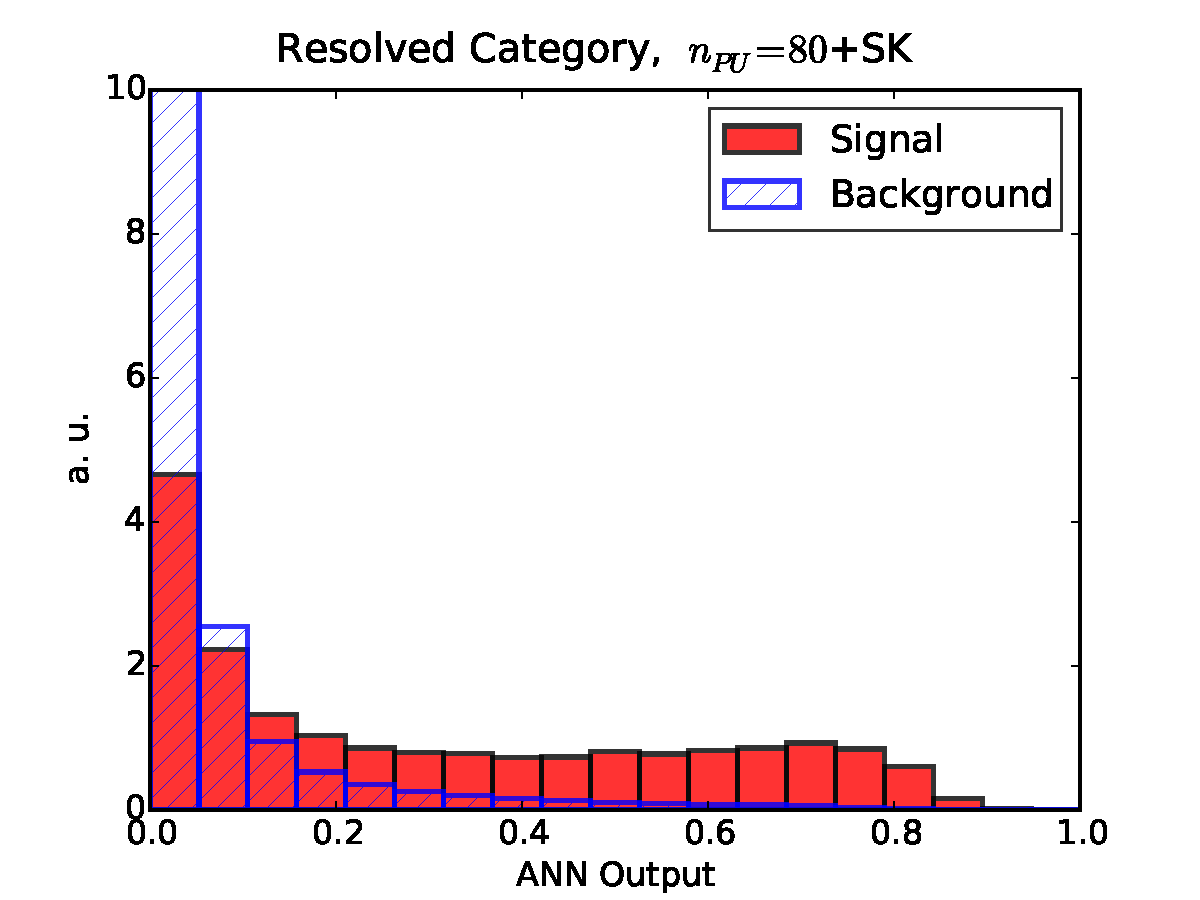
\includegraphics[width=0.49\textwidth]{plots/Resolved_disc_SKPU80.pdf}
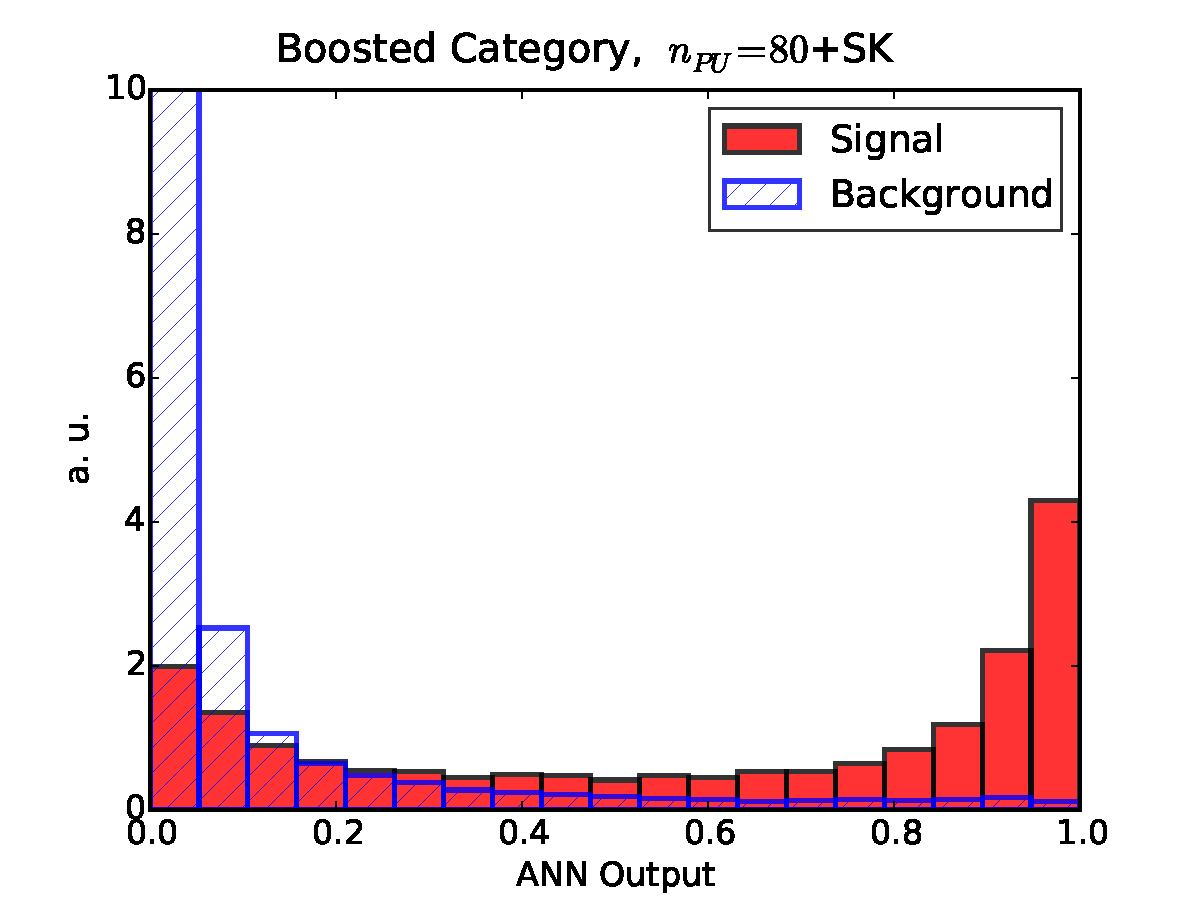
\includegraphics[width=0.49\textwidth]{plots/Boosted_disc_SKPU80.pdf}
\caption{\small Same as Fig.~\ref{fig:nnresponse},
  this time with $\la n_{\rm PU}\ra=80$ PU events per bunch crossing
  and SK subtraction, for the resolved (left) and boosted
  (right) categories.
  %
  The corresponding comparison without PU was shown in
  Fig.~\ref{fig:nnresponse}.
}
\label{fig:nnresponse_PU}
\end{center}
\end{figure}
%%%%%%%%%%%%%%%%%%%%%%%

Next we consider the number of signal and background events that
are expected at the HL-LHC as a function of the ANN discriminant -
the corresponding results without PU are those of
Fig.~\ref{fig:nev2}.
%
As we can see from Fig.~\ref{fig:nev2_PU}, the trends are
similar as in the no PU case, for instance, in the boosted
category we are left with around 200 events for the optimal value
of the ANN cut.
%
Comparing Figs.~\ref{fig:nev2} and~\ref{fig:nev2_PU}, we also observe
that the intermediate category is substantially degraded once PU
is included, since a reduced number of events fall into this
category now.

%%%%%%%%%%%%%%%%%%%%%%%%%%%%%%%%%%%%%%%%%%%%%
\begin{figure}[t]
\begin{center}
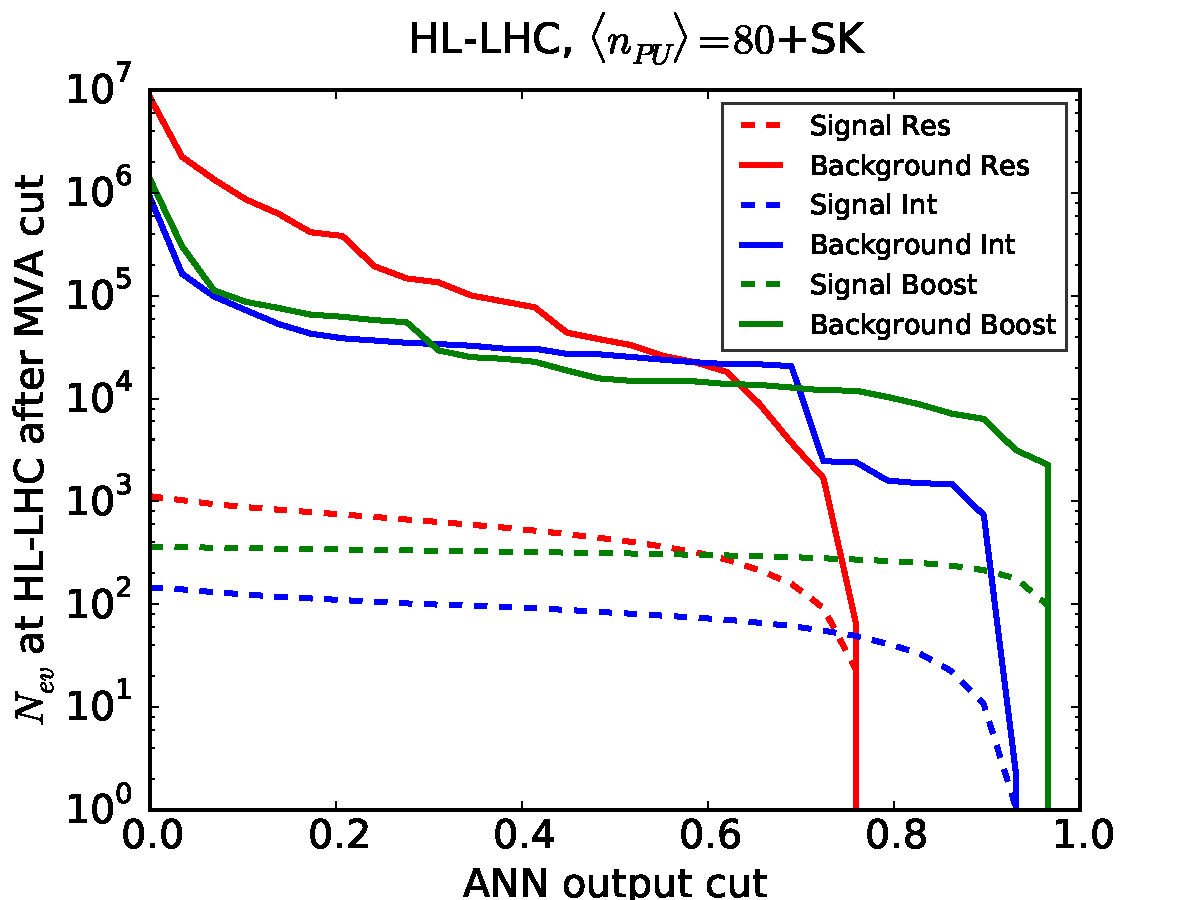
\includegraphics[width=0.65\textwidth]{plots/nev2_SKPU80.pdf}
\caption{\small Same as Fig.~\ref{fig:nev2} now
  with  $\la n_{\rm PU}\ra=80$ PU events 
  and SK subtraction.
}
\label{fig:nev2_PU}
\end{center}
\end{figure}
%%%%%%%%%%%%%%%%%%%%%%%%%%%%%%%%%%%%%

Now we can finally revisit the post-MVA signal significance,
$S/sqrt{B}$, and he signal over background ratio, $S/B$,
in the case of PU, and compare with the corresponding
no PU results shown in Fig.~\ref{fig:sb_mva}.
%

In Fig.~\ref{fig:sb_mva_PU} we show the signal significance,
$S/\sqrt{B}$, as well as the signal over background ratio,
$S/B$, as a function of the NN discriminant, in the case
of the analysis including the effects of PU
with $\la n_{\rm PU}\ra=150$.
%
The corresponding results in the case without PU were shown in
Fig.~\ref{fig:sb_mva}.
%
As can be seen, the MVA-driven enhancement is robust event in the
presence of PU, and a total signal significance of
almost $S/\sqrt{B}\simeq 3$ is also obtained in this case.
%
Therefore, we conclude that the qualitative results obtained
in the previous section are robust even in the presence
of realistic PU effects.
%
Note that no specific effort has been performed to
optimize PU subtraction (for example by tuning the value
of the patch length $a$ in {\tt SoftKiller}), so there is
certainly still room for improvement.


%%%%%%%%%%%%%%%%%%%%%%%%%%%%%%%%%%%%%%%%%%%%%%%%%%%%
%%%%%%%%%%%%%%%%%%%%%%%%%%%%%%%%%%%%%%%%%%%%%%%%%%%%
\begin{figure}[t]
\begin{center}
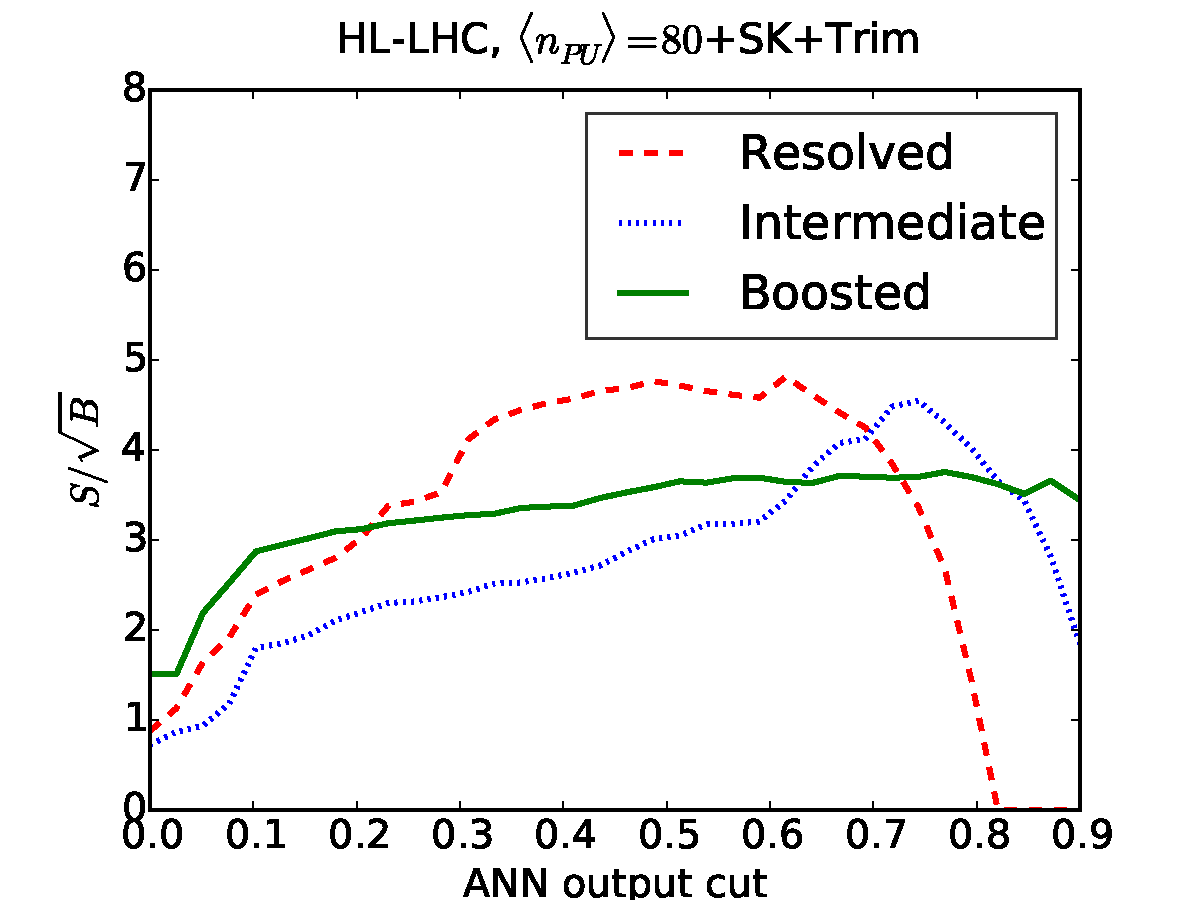
\includegraphics[width=0.48\textwidth]{plots/ssb_SKPU80.pdf}
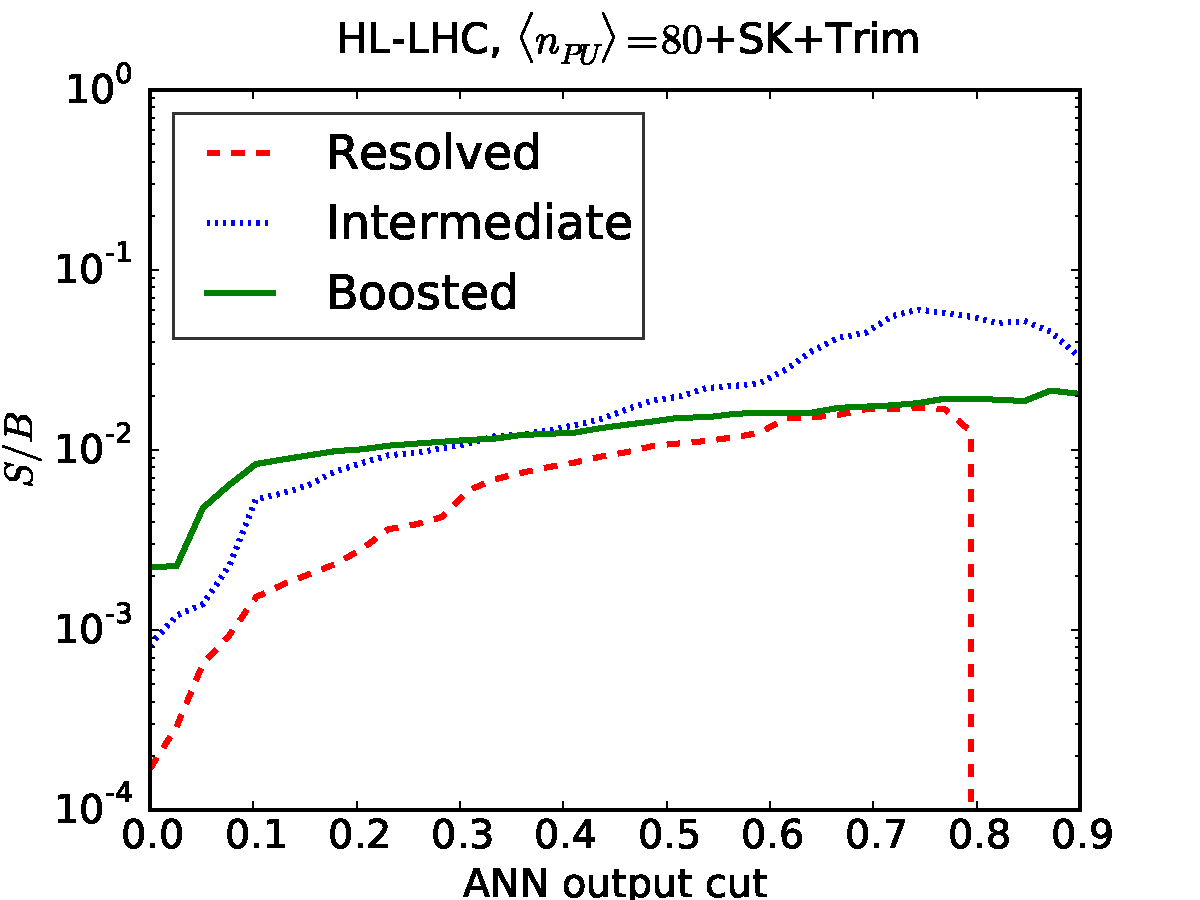
\includegraphics[width=0.48\textwidth]{plots/sb_SKPU80.pdf}
\caption{\small Same as Fig.~\ref{fig:sb_mva}
  now
  with  $\la n_{\rm PU}\ra=80$ PU events 
  and SK subtraction.
}
\label{fig:sb_mva_PU}
\end{center}
\end{figure}
%%%%%%%%%%%%%%%%%%%%%%%

To conclude, it is illustrative to quantify which of the input variables
to the MVA are most significant in the case of PU,
and compare it with the corresponding
results without PU.
%
We use the same estimator as in Sect.~\ref{sec:signalsignificance},
namely the sum
of the absolute value of all the weights connected to a given
input neuron $i$, Eq.~(\ref{eq:totweight}).
%
The results for the resolved and boosted categories are shown
on Fig.~\ref{fig:nnweights_PU}.
%
As we can see by comparing to the corresponding
results without PU in Fig.~\ref{fig:nnweights}, we see that
in the boosted category, the discrimination power of the invariant
mass of Higgs candidates is decreased and that of the various substructure
variables, in particular $C_2$ and $D^{{\rm rm}}$, is conversely
increased.
%
This reflects the fact that these substructure variables are
relatively robust against PU contamination.

In the case of the resolved category, in the case without PU the highest
values of the weight sum were found for the $p_T$ of the leading
Higgs and for the Higgs invariant masses.
%
This is also true in the case with PU, but now the rapidity difference
between the two Higgs candidates, $\Delta y_{hh}$ increases its
importance, again reflecting that this variable is relatively
insensitive to PU effects.

%%%%%%%%%%%%%%%%%%%%%%%%
\begin{figure}[t]
\begin{center}
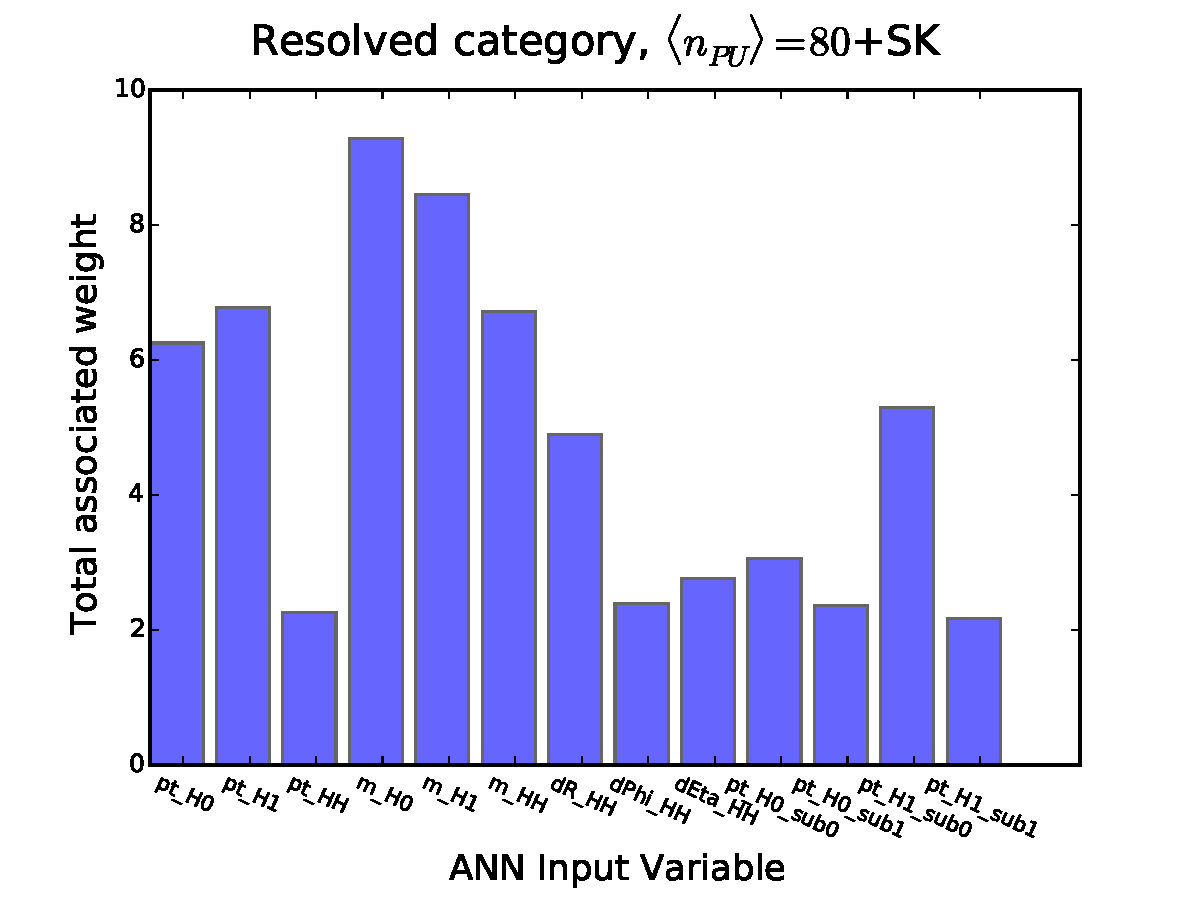
\includegraphics[width=0.49\textwidth]{plots/res_wgthist_SKPU80.pdf}
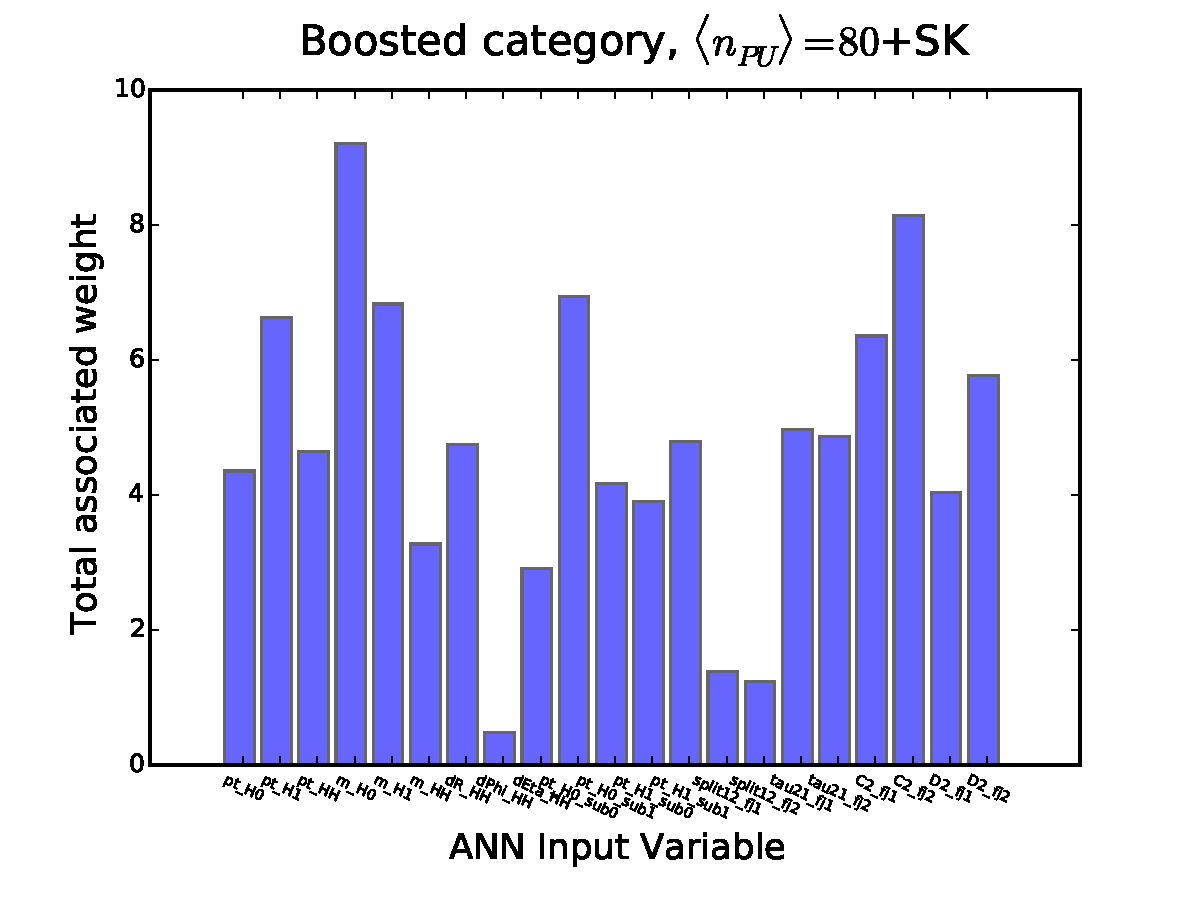
\includegraphics[width=0.49\textwidth]{plots/bst_wgthist_SKPU80.pdf}
\vspace{-0.5cm}
\caption{\small
Same as Fig.~\ref{fig:nnweights} in the case of PU.
}
\label{fig:nnweights_PU}
\end{center}
\end{figure}
%%%%%%%%%%%%%%%%%%%%%%%




\subsection{Combined results}

Finally, we now combine the three categories, resolved,
intermediate and boosted, and determine the signal
significance taking into account all event topologies.
%
First of all, in Table~\ref{table:cutflowMVA_PU}
we provide the  the number of signal and
    background events at the HL-LHC, as well as the $S/\sqrt{B}$ and $S/B$,
    for both the cut-based analysis (corresponding
    to $y_{\rm cut}=0$) and after the
    optimal MVA cut.
    %
    These numbers corresponding to the simulations
    with $\la n_{\rm PU}\ra=80$
    and SK subtraction.
    %
    The corresponding results without PU were collected
    in Table.~\ref{table:cutflowMVA}.
    %
    The value of the optimal MVA cut $y_{\rm cut}$ is determined
    as the one leading to highest signal significance, with
    the constraint that number of MC events left is still large
    enough to tame statistical fluctuations.


%%%%%%%%%%%%%%%%%%%%%%%%%%%%%%%%%%%%%%%%%%%%%%%%%%%%%
\begin{table}[t]
  \centering
  \begin{tabular}{c|c|c|c||c|c|c|c}
    \hline
    \multicolumn{8}{c}{Boosted category, $\la n_{\rm PU}\ra=80$+SK}\\
    \hline
    \hline
    \multicolumn{4}{c||}{no MVA cut} & \multicolumn{4}{c}{optimal MVA cut}\\
    \multicolumn{4}{c||}{$y_{\rm cut}=0$} & \multicolumn{4}{c}{$y_{\rm cut}=0.84$}\\
    \hline
    \multicolumn{2}{c|}{$N_{\rm ev}$} &  $S/\sqrt{B}$  & $S/B$
    & \multicolumn{2}{c|}{$N_{\rm ev}$} &  $S/\sqrt{B}$  & $S/B$\\
        Signal & Back   &     &   &  Signal & Back   &     &    \\
    \hline
    362  &  $1.4\cdot 10^6$     & 0.31       &  $3\cdot 10^{-4}$ &
    248     &   7250             &  2.9       & 0.034 \\
        \hline
  \end{tabular}
   $\,$\\
  \vspace{0.4cm}
  \noindent
  \begin{tabular}{c|c|c|c||c|c|c|c}
    \hline
    \multicolumn{8}{c}{Intermediate category,  $\la n_{\rm PU}\ra=80$+SK}\\
    \hline
    \hline
    \multicolumn{4}{c||}{no MVA cut} & \multicolumn{4}{c}{optimal MVA cut}\\
    \multicolumn{4}{c||}{$y_{\rm cut}=0$} & \multicolumn{4}{c}{$y_{\rm cut}=0.72$}\\
    \hline
    \multicolumn{2}{c|}{$N_{\rm ev}$} &  $S/\sqrt{B}$  & $S/B$
    & \multicolumn{2}{c|}{$N_{\rm ev}$} &  $S/\sqrt{B}$  & $S/B$\\
        Signal & Back   &     &   &  Signal & Back   &     &    \\
    \hline
    146  &    $9\cdot 10^5$   & 0.15        &  $2\cdot 10^{-4}$      &
  53  &  2547        & 1.1        &  0.02 \\
        \hline
  \end{tabular}
    $\,$\\
  \vspace{0.4cm}
  \noindent
  \begin{tabular}{c|c|c|c||c|c|c|c}
    \hline
    \multicolumn{8}{c}{Resolved category,  $\la n_{\rm PU}\ra=80$+SK}\\
    \hline
    \hline
    \multicolumn{4}{c||}{no MVA cut} & \multicolumn{4}{c}{optimal MVA cut}\\
    \multicolumn{4}{c||}{$y_{\rm cut}=0$} & \multicolumn{4}{c}{$y_{\rm cut}=0.49$}\\
    \hline
    \multicolumn{2}{c|}{$N_{\rm ev}$} &  $S/\sqrt{B}$  & $S/B$
    & \multicolumn{2}{c|}{$N_{\rm ev}$} &  $S/\sqrt{B}$  & $S/B$\\
        Signal & Back   &     &   &  Signal & Back   &     &    \\
    \hline
  1123  &    $8.5\cdot 10^6$   & 0.40       &  $1.3\cdot 10^{-4}$       &
  432  &  $3\cdot 10^4$        &   2.5      & 0.15 \\
        \hline
  \end{tabular}
  \caption{\small The results for the number of signal and
    background events
    at the HL-LHC for both the cut-based analysis and after the
    optimal MVA cut, as well as the $S/\sqrt{B}$ and $S/B$
    values in the two cases, in the case of $\la n_{\rm PU}\ra=80$
    and SK subtraction.
    %
    The corresponding results without PU were collected
    in Fig.~\ref{table:cutflowMVA}.
        \label{table:cutflowMVA_PU}
  }
\end{table}
%%%%%%%%%%%%%%%%%%%%%%%%%%%%%%%%%%%%%%%%%%%%%%%%%%%%%

From Table~\ref{table:cutflowMVA_PU} we see that, thanks
to the MVA, we can improve the signal significance and the
signal over background ratio from 0.31 and $3\cdot 10^{-4}$
(0.40 and $1.3\cdot 10^{-4}$) up to 2.9 and 0.034 (2.5 and 0.15)
in the boosted (resolved) category.
%
The intermediate category exhibits a lower value of $S/\sqrt{B}$
for the optimal $y_{\rm cut}$ value, around unity.
%
We thus conclude that the boosted category is the most promising
one for the study of Higgs pair production in the $b\bar{b}b\bar{b}$
at the HL-LHC, with however useful information also provided
by the resolved category.

Adding in quadrature the signal significance from the three
(exclusive) categories, our final combined result is
\be
\lp \frac{S}{\sqrt{B}}\rp_{\rm tot} \simeq 4.0 \, ,
\ee
far above the threshold for {\it evidence}, and close to the
requirement for {\it discovery}.
%
In addition, it should be emphasized that there is still
room for improvement, in particular by means of a tailored
study dedicated to optimize PU subtraction in this process.



In summary, in this section we have demonstrated the robustness
of our results under the presence of PU conditions as those
expected at the HL-LHC.
%
With a signal significance of $S/\sqrt{B}\sim 4$, is clear that
the $b\bar{b}b\bar{b}$ final state can be used to claim evidence
for Higgs pair production at the HL-LHC without the need
to combine with any other final state.
%
It will be important now to quantify the precision of
a extraction of the Higgs trilinear coupling $\lambda$ using
the techniques presented here, but this is left for future work.
